% Sparse Autoencoders Are a Shared Coordinate System for Symbolic Matching -- NAACL submission draft.
% Build: tectonic -X compile main.tex   (XeTeX; CJK/Arabic glyphs shown if a font is found)
%     or pdflatex + bibtex (glyphs fall back to romanisation).
\documentclass[11pt]{article}

% Change "review" to "final" for the camera-ready version.
\usepackage[review]{acl}

\usepackage{iftex}
\newif\ifcjk \newif\ifarab
\ifXeTeX
  \usepackage[no-math]{fontspec}
  \IfFontExistsTF{Noto Sans CJK SC}{\newfontfamily\cjkfont{Noto Sans CJK SC}\cjktrue}{%
    \IfFontExistsTF{Droid Sans Fallback}{\newfontfamily\cjkfont{Droid Sans Fallback}\cjktrue}{\cjkfalse}}
  \IfFontExistsTF{Noto Sans Arabic}{\newfontfamily\arabfont[Script=Arabic]{Noto Sans Arabic}\arabtrue}{%
    \IfFontExistsTF{Droid Arabic Kufi}{\newfontfamily\arabfont[Script=Arabic]{Droid Arabic Kufi}\arabtrue}{\arabfalse}}
  \usepackage{times}
\else
  \usepackage[T1]{fontenc}
  \usepackage[utf8]{inputenc}
  \usepackage{times}
  \cjkfalse \arabfalse
\fi
% \zh{<characters>}{<romanisation>}: characters when a font is available, else the romanisation.
\newcommand{\zh}[2]{\ifcjk{\cjkfont #1}\else #2\fi}
\newcommand{\arb}[2]{\ifarab{\arabfont #1}\else #2\fi}

\usepackage{latexsym}
\usepackage{microtype}
\usepackage{inconsolata}
\usepackage{graphicx}
\usepackage{booktabs}
\usepackage{makecell}
\usepackage{amsmath}
\usepackage{amssymb}
\usepackage{xspace}
\usepackage{float}

\newcommand{\method}{SAE\mbox{-}IDF\xspace}
\newcommand{\saemean}{SAE\textsubscript{unw}\xspace}
\newcommand{\pcone}{Dense\textsubscript{$-$PC1}\xspace}
\newcommand{\R}{\mathbb{R}}
\newcommand{\idf}{\mathrm{idf}}
\newcommand{\df}{\mathrm{df}}
\DeclareMathOperator*{\argmax}{arg\,max}
\setlength{\textfloatsep}{10pt plus 2pt minus 2pt}
\setlength{\floatsep}{8pt plus 2pt minus 2pt}
\setlength{\abovecaptionskip}{5pt}
\setlength{\dbltextfloatsep}{10pt plus 2pt minus 2pt}

\title{Sparse Autoencoders Are a Shared Coordinate System\\for Symbolic Matching}

\author{Anonymous NAACL submission \\
  % Xiaocong Yang \\ University of Illinois Urbana-Champaign \\ \texttt{xy51@illinois.edu}
}

\begin{document}
\maketitle

\begin{abstract}
Human knowledge is encoded in many mutually incompatible symbolic systems---ontologies, knowledge graphs, database schemas, programming languages, proof assistants---that name the same things differently.
Aligning them is a prerequisite for a general-purpose symbolic layer over large language models, yet alignment is still studied one kind of system at a time, with methods that lean on surface strings or on supervised pairs.
We show that the sparse-autoencoder (SAE) features of a pretrained LLM form a shared coordinate system in which symbols from all of these systems can be matched without training.
\method represents a symbol by the SAE features that its own system-internal context activates, re-weights every feature by its rarity (inverse document frequency), and matches by cosine.
On ten tasks spanning formal mathematics (miniF2F, Lean~4 to Isabelle, Metamath and HOL Light), code (XLCoST), table schemas (Valentine), knowledge graphs (OAEI Common-KG) and cross-lingual ontologies (MultiFarm), \method beats the dense hidden state of the same model on every task (+0.01 to +0.45 MRR), beats common-direction-removed dense on 15 of 16 comparisons, and is ahead of an off-the-shelf multilingual retriever (BGE-M3) on 12 of 16; the gains over the model's own states are largest where notations differ most (Lean~4 to Metamath: MRR 0.66 vs.\ 0.21).
Rarity weighting is what makes the sparse basis useful: without it the same features trail dense on 13 of 16 comparisons; with it \method beats dense in all 39 settings of layer, SAE width, sparsity, model size (2B to 27B) and model family we tried, and on a second model family (Llama-3.1-8B) run over the whole main table it beats dense on 11 of 12 rows, although there its margin over common-direction-removed dense narrows to a tie on knowledge-graph and cross-lingual terms.
Because the cosine decomposes over named features, every match is readable: the Chinese term \zh{费用}{\emph{feiyong}} matches ``fee for conference'' through a single feature for ``fees and payment structures''.
We argue that an LLM's own feature dictionary is a candidate substrate for aligning and merging existing symbolic systems into a universal symbolic backbone.
\end{abstract}

\section{Introduction}
\label{sec:intro}

Knowledge is written down in thousands of symbolic systems that do not share a vocabulary: a disease is \emph{Duodenal Atresia} in one biomedical ontology and an opaque identifier in the next; a competition problem is a Lean~4 \texttt{theorem} in one proof assistant and a string of \texttt{\$e} hypotheses in Metamath; a table column is \texttt{src\_id} here and \texttt{SRI} there.
Putting such systems in correspondence is a classic problem in several communities---ontology matching \citep{euzenat2013ontology}, schema matching \citep{rahm2001survey}, entity alignment \citep{sun2020benchmarking}, cross-language code retrieval \citep{zhu2022xlcost}---but each solves it for its own kind of system, with lexical matchers tuned to its naming conventions or with models trained on aligned pairs.
We call the task \emph{symbolic matching}, whatever the kind of system; its output for one pair of systems is an \emph{alignment}, and composing alignments across many systems into one symbol inventory is \emph{merging}.

The question matters beyond any one community.
\citet{yang2026generative} argues that once LLMs act as agents, interpretability must become \emph{generative}---an inference pass should expose checkpoints that are natively human-readable and causally intervenable---and proposes neuro-symbolic models, whose symbolic components serve as those checkpoints, as the instance.
The first obstacle that paper names is a universal, general-purpose symbolic system.
Writing one by hand failed: Cyc absorbed a person-century of effort for about $10^5$ concepts \citep{lenat1995cyc}.
The proposed alternative is to align, merge and extend the symbolic systems that already exist; alignment across \emph{heterogeneous} systems is the first operation that route needs, and no single method today spans the kinds of systems involved.

A pretrained LLM reads all of these notations, so its hidden states are a candidate common space, but they are anisotropic, dominated by directions shared by all inputs \citep{ethayarajh2019contextual, mu2018allbutthetop}.
Sparse autoencoders (SAEs) decompose the same states into a large dictionary of sparsely active, individually interpretable features \citep{bricken2023monosemanticity, cunningham2024sparse, templeton2024scaling}, available for every layer of Gemma~2 and Llama~3.1 \citep{lieberum2024gemmascope, he2024llamascope} and shared across languages and modalities \citep{templeton2024scaling, brinkmann2025grammatical}---exactly what a shared symbol space needs.
Whether SAE features are \emph{useful} beyond interpretation is contested \citep{kantamneni2025sparse}.

\paragraph{This paper.}
We propose \method, a training-free procedure for symbolic matching in an LLM's SAE feature space (Figure~\ref{fig:pipeline}).
Each symbol is read in \emph{native views} drawn from its own system---the program, the formal statement, the column's values, the class's instances, the term's axioms---so nothing is generated and no aligned pairs are used; the SAE encodes the hidden states at the symbol's tokens, the sparse codes are averaged into one vector $a(s)\in\R^F$, each coordinate is multiplied by the feature's inverse document frequency over the symbols being matched, and candidates are ranked by cosine.
The idea is TF-IDF \citep{sparckjones1972statistical} with SAE features in place of words, identical for every kind of system.

\paragraph{Evidence.}
With one model and one setting (Gemma-2-9B, layer~20, 131k-feature Gemma Scope SAE), \method beats the dense hidden state of the same model, pooled identically, on all 16 main-table comparisons across five kinds of system (+0.01 to +0.45 MRR), is ahead of dense with its first principal component removed on 15 of 16 (significantly on 12), and is ahead of an off-the-shelf multilingual retriever, BGE-M3 \citep{chen2024bge}, on 12 of 16, which is stronger only on two formal-mathematics pairs, Valentine and NELL $\to$ DBpedia (Section~\ref{sec:results}).
The gains are largest where surface forms differ most: Lean~4 to Metamath (0.661 vs.\ 0.210) and to HOL Light (0.898 vs.\ 0.539).
Removing the rarity weighting removes the gain: the unweighted code trails dense on 13 of 16 comparisons; with it, \method beats dense in all 39 configurations of layer, width, sparsity, model size (2B to 27B) and model family we ran, and a second model family (Llama-3.1-8B) run over the whole main table beats dense on 11 of 12 rows, with the lead over common-direction-removed dense narrowing to a tie on knowledge-graph and cross-lingual terms (Section~\ref{sec:ablation}).
Every match decomposes exactly into the features the two symbols share (Section~\ref{sec:interp}): without weighting, one feature for ``mathematical or programming notation'' dominates 99\% of correct matches; with weighting, matches rest on rare, named concepts.

\paragraph{Contributions.}
(i)~A training-free alignment primitive that applies unchanged to five kinds of symbolic system, evaluated on full datasets against string, dense and common-direction-removed baselines.
(ii)~An ablation showing that the rarity weighting, not the sparse basis alone, carries the result, across 39 settings, two model families and three kinds of system.
(iii)~A feature-level account of \emph{why} it works: rule-selected case studies, a column-type split that locates where a symbolic rule should take over from the neural signature, and merge tests showing that pairwise alignments compose---together, a first test of an LLM's feature dictionary as the substrate for the ``align and merge existing systems'' route to a universal symbolic backbone.

\begin{figure*}[t]
  \centering
  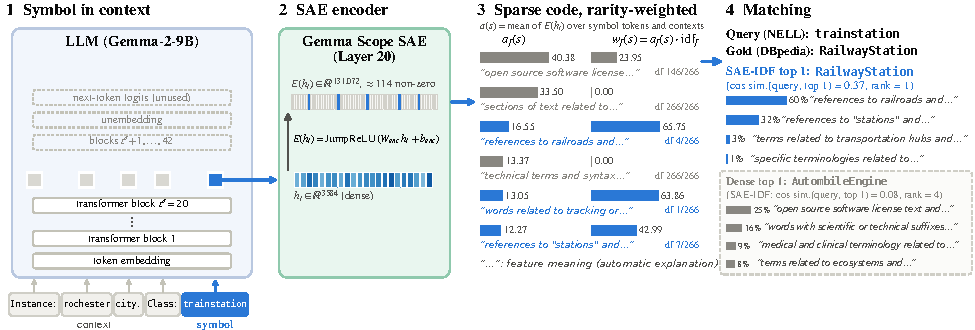
\includegraphics[width=0.9\textwidth]{figures/fig_pipeline.pdf}
  \caption{\method. (1)~A symbol $s$ is read in views from its own system, evidence first and symbol last; the LM reads the whole view and only the hidden states at the symbol's tokens are kept (for a program, formal statement or table column the whole text is the symbol). (2)~Each kept state is SAE-encoded and the codes are averaged into one sparse vector $a(s)$ over $F$ features. (3)~Each coordinate is multiplied by its feature's inverse document frequency over the symbols being matched, which sends features that fire on almost every symbol to zero, and candidates are ranked by cosine.}
  \label{fig:pipeline}
\end{figure*}

\section{\method}
\label{sec:method}

\paragraph{Setup.}
For each query symbol $s$ of a source system $A$ we rank a candidate set $C(s)$ from a target system $B$ so that its counterpart comes first.
Let $h_t\in\R^d$ be the residual stream of a causal language model at layer $\ell$ and token position $t$ when it reads a text, and let $E:\R^d\to\R^F_{\ge 0}$ be the encoder of a sparse autoencoder with $F$ features trained on that layer.
In the main experiments the model is Gemma-2-9B \citep{gemmateam2024gemma2} at $\ell=20$ of 42 ($d=3{,}584$) and the SAE is the Gemma Scope JumpReLU SAE with $F=131{,}072$ and average $L_0$ of 114 \citep{lieberum2024gemmascope, rajamanoharan2024jumping}.

\paragraph{1. Native views.}
Each symbol $s$ has views $v_1(s),\dots,v_m(s)$ taken from its own system; nothing is generated.
A program, a formal statement or a table column is its own single view ($m=1$); a column is written as its name followed by 16 sampled cell values.
For classes and terms, each view concatenates one piece of system-internal evidence $e_j(s)$ with the symbol, evidence first:
\texttt{Instance: Earth mass. Class: Mass} (Common-KG) or \texttt{domain} \zh{投稿}{\emph{tougao}}\texttt{. Term:} \zh{有标题}{\emph{you biaoti}} (an axiom of a MultiFarm term in its own language).
The model reads the whole view, but only the hidden states at the symbol's own token positions $T_j(s)$ are kept (all positions when the symbol is the whole text); the symbol comes last because the model is causal, so its tokens see the evidence.
Synonyms are never used as evidence (across systems a synonym is often the other side's label); views are capped at 16 per symbol.

\paragraph{2. Sparse code.}
Every kept token is SAE-encoded first and the codes are averaged afterwards, over tokens and then views:
\begin{equation}
  a(s) \;=\; \frac{1}{m}\sum_{j=1}^{m}\frac{1}{|T_j(s)|}\sum_{t\in T_j(s)} E(h_t)\;\in\R^{F}.
  \label{eq:code}
\end{equation}
The order matters: the JumpReLU threshold is applied per token, so averaging hidden states before encoding would drop any feature that fires on only part of a symbol.
$a(s)$ is the symbol's \emph{sparse code}, one non-negative coefficient per feature, most of them zero.

\paragraph{3. Rarity weighting.}
Over a reference collection $D$ of $N$ symbols, let $\df(f)=|\{u\in D : a_f(u)>0\}|$ be the number of symbols on which feature $f$ fires.
Each coefficient is multiplied by its feature's inverse document frequency,
\begin{equation}
  w(s) = a(s)\odot\idf\in\R^F,\;\; \idf_f=\Big[\log\tfrac{N}{1+\df(f)}\Big]_+ .
  \label{eq:idf}
\end{equation}
$D$ is the candidate pool for miniF2F, XLCoST and Valentine, and all symbols of both systems for the ontology and knowledge-graph tasks; a feature that fires on every symbol gets weight zero.

\paragraph{4. Matching.}
Candidates are ranked by the cosine of the weighted vectors, $\hat t(s)=\argmax_{t\in C(s)}\cos\big(w(s),w(t)\big)$.
The compared objects are the sparse codes: the cosine runs over the $F$ coordinates and the features' decoder directions never enter the score; a feature is a named coordinate axis that both systems share because the same model and SAE read both.
The cosine decomposes exactly over shared features, $\cos(w(s),w(t))=\sum_f c_f$ with $c_f=w_f(s)\,w_f(t)/(\|w(s)\|\,\|w(t)\|)$, which is what makes every match readable (Section~\ref{sec:interp}).

\paragraph{Baselines.}
All baselines use exactly the same views and token positions.
\emph{Dense} is the hidden state averaged as in Eq.~\ref{eq:code} without the SAE.
\emph{\pcone} additionally subtracts the mean of the dense vectors over $D$ and removes their projection onto the first principal direction $u_1$ of $D$, $(I-u_1u_1^\top)(d-\mu)$, the common-direction removal of \citet{mu2018allbutthetop} and \citet{arora2017simple}; it is the strongest control we found.
\emph{\saemean} is the unweighted code $a(s)$, which isolates the sparse basis from the weighting.
\emph{Strings} is the best of word TF-IDF \citep{sparckjones1972statistical}, character 3--5-gram TF-IDF and BM25 \citep{robertson2009probabilistic} over the surface strings of the same views, chosen per task in the strings' favour (Appendix~\ref{app:benchmarks}); since \method is TF-IDF over SAE features, TF-IDF over strings separates the features from the weighting.
\emph{Retriever}: BGE-M3 \citep{chen2024bge}, a multilingual embedding model trained for retrieval, on the same view texts with the same controls (Appendix~\ref{app:embed}).
Every similarity is a cosine.

\section{Benchmarks}
\label{sec:benchmarks}

The five kinds of system were chosen to differ as much as possible in notation, with every symbol having context native to its own system (Table~\ref{tab:benchmarks}, Appendix~\ref{app:benchmarks}); every run uses the full test data and the benchmark's own metric code where one exists.

\paragraph{Protocols.}
miniF2F \citep{zheng2022minif2f}: from the Lean~4 port \citep{yang2023minif2flean4} we retrieve each problem's statement in another prover among all statements of that prover, with theorem names, proofs, comments and labels stripped so that nothing identifies a problem without reading the mathematics.
XLCoST \citep{zhu2022xlcost}: the official protocol and evaluator (the pool contains the query's own row, a free first hit); MRR and Precision@6 averaged over the seven query languages.
Valentine \citep{koutras2021valentine}: all 551 fabricated joinable and unionable pairs, scored with Valentine's F1 (one-to-one assignment) and MRR.
Common-KG \citep{fallatah2020gold}: 129 NELL--DBpedia reference pairs (a partial gold standard) and 304 YAGO--Wikidata pairs; classes without instances match on their label alone.
MultiFarm \citep{meilicke2012multifarm}: foreign-language terms against the English terms of a \emph{different} conference ontology, so that neither language nor ontology is shared.
The metric is MRR unless stated; Appendix~\ref{app:benchmarks} gives view formats and the reference collections used for $\df$.

\paragraph{Appendix tasks.}
Bio-ML NCIT $\to$ DOID \citep{he2022bioml} and OAEI Anatomy \citep{bodenreider2005mice}, where about half of the gold pairs have identical labels, and PubChem SMILES / IUPAC / InChI \citep{kim2023pubchem}, notations the model cannot read, are reported in Appendix~\ref{app:tasks}; drug brand $\to$ generic names were dropped because both names share one FDA record, so neither side has independent native context (Appendix~\ref{app:generated}).

\section{Results}
\label{sec:results}

\begin{table*}[t]
  \centering\footnotesize
  \setlength{\tabcolsep}{4pt}
  \begin{tabular}{@{}llrrrrrr@{}}
\toprule
Task & Metric & Strings & Dense & \makecell{Dense,\\PC1 rm.} & \makecell{SAE\\unweighted} & \textbf{SAE-IDF} & $\Delta$ dense \\
\midrule
\multicolumn{8}{@{}l}{\textit{Formal mathematics (miniF2F)}} \\
\quad Lean 4 $\to$ Isabelle & MRR & 0.825 & 0.912 & 0.926 & 0.882 & \textbf{0.961} & +0.05 \\
\quad Lean 4 $\to$ Metamath & MRR & 0.615 & 0.210 & 0.151 & 0.095 & \textbf{0.661} & +0.45 \\
\quad Lean 4 $\to$ HOL Light & MRR & 0.741 & 0.539 & 0.531 & 0.493 & \textbf{0.898} & +0.36 \\
\multicolumn{8}{@{}l}{\textit{Code (XLCoST, program level)}} \\
\quad 7 languages, mean & MRR$^\dagger$ & \textbf{0.468} & 0.454 & 0.452 & 0.449 & 0.464 & +0.01 \\
\quad 7 languages, mean & P@6$^\dagger$ & \textbf{0.745} & 0.680 & 0.678 & 0.673 & 0.732 & +0.05 \\
\multicolumn{8}{@{}l}{\textit{Table schemas (Valentine, 551 pairs)}} \\
\quad source $\to$ target columns & F1 & -- & 0.533 & 0.534 & 0.458 & \textbf{0.614} & +0.08 \\
\quad source $\to$ target columns & MRR & -- & 0.766 & 0.761 & 0.685 & \textbf{0.856} & +0.09 \\
\multicolumn{8}{@{}l}{\textit{Knowledge graphs (OAEI Common-KG)}} \\
\quad NELL $\to$ DBpedia & MRR & 0.936 & 0.931 & 0.957 & 0.938 & \textbf{0.976} & +0.04 \\
\quad YAGO $\to$ Wikidata & MRR & 0.899 & 0.860 & 0.932 & 0.872 & \textbf{0.962} & +0.10 \\
\multicolumn{8}{@{}l}{\textit{Cross-lingual ontologies (MultiFarm)}} \\
\quad Chinese $\to$ English & MRR & 0.230 & 0.650 & \textbf{0.760} & 0.404 & 0.754 & +0.10 \\
\quad Russian $\to$ English & MRR & 0.234 & 0.644 & 0.751 & 0.252 & \textbf{0.765} & +0.12 \\
\quad Arabic $\to$ English & MRR & 0.238 & 0.595 & 0.702 & 0.225 & \textbf{0.722} & +0.13 \\
\bottomrule
\end{tabular}

  \caption{Main results with native context. Gemma-2-9B, layer 20, Gemma Scope 131k SAE. Bold: best method per row. $\Delta$ dense: \method minus Dense. $^\dagger$XLCoST official metrics averaged over the seven query languages (per-language results in Appendix~\ref{app:xlcost}); Strings is word TF-IDF there. Valentine has no comparable string baseline.}
  \label{tab:main}
\end{table*}

Table~\ref{tab:main} gives the main results (plotted in Figure~\ref{fig:main}, Appendix~\ref{app:tasks}).
\method beats the dense hidden state of the same model on every task, by +0.01 (XLCoST) to +0.45 MRR (Lean~4 $\to$ Metamath).
It is ahead of \pcone and of strings everywhere except on XLCoST (word TF-IDF marginally ahead) and MultiFarm Chinese (\pcone ahead by 0.006), and ahead of the BGE-M3 retriever on 12 of the 16 comparisons.

\paragraph{The gain tracks notational distance.}
Isabelle statements resemble Lean~4 (dense 0.912, \method 0.961); Metamath and HOL Light read very differently, dense collapses there (0.210, 0.539) and \method keeps 0.661 and 0.898.
On MultiFarm, where source and target share neither script nor ontology, strings are near useless (0.23) and \method gains +0.10 to +0.13 over dense.

\paragraph{Code: shared identifiers favour strings.}
XLCoST programs are translations that keep their identifiers, so word TF-IDF is a strong baseline (0.468 official MRR over seven languages).
\method matches it within 0.01, beats dense in all seven languages (also without the free hit, Appendix~\ref{app:exclude}), and recovers most of dense's deficit on Precision@6 (0.732 vs.\ 0.680; strings 0.745); surface form wins only where the two notations share the most.

\paragraph{Table schemas.}
On Valentine \method has the best F1 (0.614 vs.\ 0.533 dense) and MRR (0.856 vs.\ 0.766) and leads dense in every dataset family except Magellan, where every method scores 1.0 (Appendix~\ref{app:valentine} compares four column layouts).

\paragraph{A trained retriever.}
BGE-M3, a 568M-parameter embedding model trained for multilingual retrieval, leads \method on Lean~4 $\to$ Metamath (0.819 vs.\ 0.661), $\to$ HOL Light (0.967 vs.\ 0.898), Valentine (F1 0.645 vs.\ 0.614) and narrowly on NELL $\to$ DBpedia; \method is ahead everywhere else, by +0.04 to +0.05 on cross-lingual terms, +0.05 on YAGO $\to$ Wikidata, +0.03 on XLCoST and +0.10 to +0.21 on the biomedical appendix tasks (Appendix~\ref{app:embed}).
The comparison is not like for like (the retriever was trained on paired data; \method reads an untrained base model), but it bounds what the training-free route gives up: nothing on 12 of 16 comparisons.

\paragraph{The common-direction control, and the appendix tasks.}
Removing the first principal component recovers much of the gap on ontology and knowledge-graph terms, whose dense vectors share a large common component, and nothing on code, formal statements and tables, so \method's advantage does not reduce to anisotropy removal \citep{ethayarajh2019contextual, mu2018allbutthetop}; the next two sections take it apart.
A paired bootstrap over queries puts every gain over dense at $p<0.004$ and the gain over \pcone at $p<0.01$ on 12 of the 16 comparisons; on the three MultiFarm pairs and NELL $\to$ DBpedia the two are within noise (Appendix~\ref{app:significance}).
On Bio-ML (0.817 vs.\ 0.701 dense, 0.779 strings) and Anatomy (0.886 vs.\ 0.812, 0.734) \method leads as well; PubChem is at chance for every method (Appendix~\ref{app:tasks}).

\section{Ablations}
\label{sec:ablation}

\paragraph{Rarity weighting is the active ingredient.}
Dropping the idf factor leaves \saemean, the unweighted code $a(s)$.
The sparse basis alone does not help: \saemean trails dense on 13 of the 16 main-table comparisons and leads by at most 0.012 on the other three.
The idf factor then lifts every task, by +0.01 on XLCoST to +0.57 MRR on Metamath; Section~\ref{sec:interp} shows why: without weighting, a handful of features that fire on nearly every token dominate every cosine.

\begin{figure*}[t]
  \centering
  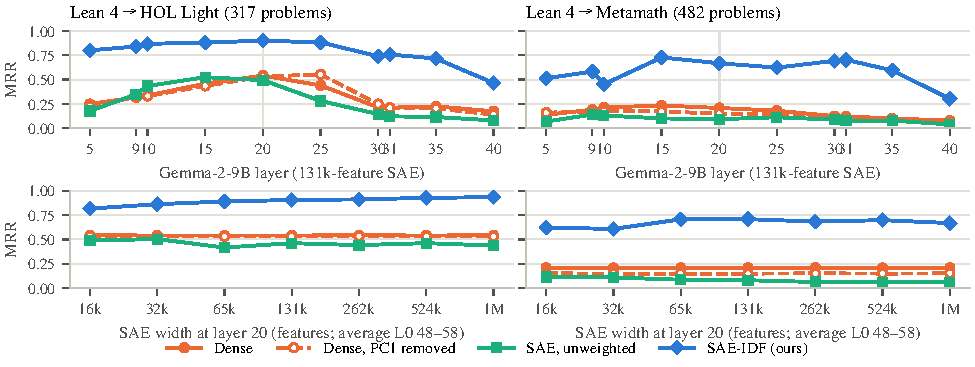
\includegraphics[width=\textwidth]{figures/fig_ablation.pdf}
  \caption{Layer sweep (top; 131k-feature SAE at each layer) and SAE-width sweep at matched sparsity (bottom; layer 20, average $L_0$ 48--58) on miniF2F Lean~4 $\to$ HOL Light and $\to$ Metamath. \method beats every baseline at every layer and width; the unweighted code tracks or trails dense.}
  \label{fig:ablation}
\end{figure*}

\paragraph{Layer, width, sparsity, model size, model family.}
We sweep the remaining choices on the two tasks where \method beats string matching by the widest margins, Lean~4 $\to$ HOL Light and $\to$ Metamath (Figure~\ref{fig:ablation}; all numbers in Appendix~\ref{app:ablation}).
Across all 39 configurations---10 layers of Gemma-2-9B; seven Gemma Scope widths from 16k to 1M features, at matched sparsity and at each width's canonical sparsity; eight sparsity levels ($L_0$ 11--276) at 131k; three widths of Gemma-2-2B; five Gemma-2-27B settings; and six Llama Scope SAEs on Llama-3.1-8B \citep{he2024llamascope, grattafiori2024llama3}---\method beats both dense and \pcone on both tasks, by +0.18 to +0.55 MRR over dense on HOL Light and +0.08 to +0.58 on Metamath, and beats \saemean in all 78 runs, by +0.11 to +0.66.
With sparsity held nearly fixed, \method rises with every doubling of the dictionary on HOL Light (0.817 at 16k to 0.935 at 1M) and levels off from 65k--131k on Metamath, while \saemean drifts \emph{down} as the dictionary widens.
This fits \emph{feature splitting} \citep{bricken2023monosemanticity, templeton2024scaling}: a wider dictionary splits concepts into more, rarer features, which help only once rarity is weighted.
Repeating both sweeps on Common-KG and MultiFarm (Figure~\ref{fig:sweepkg}, Appendix~\ref{app:ablation}) gives the same verdict against dense and the unweighted code---\method is ahead in all 45 (task, setting) pairs---but a closer race with \pcone, which is ahead at several settings on YAGO and MultiFarm, where width also helps less (MultiFarm peaks at 65k features).
The effect holds from 2B to 27B parameters (Gemma-2-27B, layer 22: 0.939 and 0.738 against dense 0.41 and 0.20) and for a second model family: with Llama-3.1-8B and Llama Scope, \method beats dense in all six miniF2F configurations (Table~\ref{tab:llama}), a middle layer (15 of 32) is again best, and the gap is smallest on Metamath, where Llama's dense state is a far stronger baseline than Gemma's (0.646 vs.\ 0.210).
On the whole main table (Table~\ref{tab:llamamain}) Llama-3.1-8B beats dense on 11 of 12 rows (all but XLCoST MRR) and \pcone on 9, the knowledge-graph and cross-lingual tasks being the close ones; at Llama's earlier layers 8 and 12 \method is ahead of \pcone on both Common-KG pairs (Table~\ref{tab:llamakg}), so that tie is a layer choice.
Among weightings, idf over the matched collection beats an idf from Pile activation densities on every task (0.661 vs.\ 0.190 on Metamath): which features count as generic depends on the two systems being matched (Table~\ref{tab:weightings}).

\paragraph{Generated contexts do not work as well.}
Before settling on native views we described each symbol with LLM-written sentences (one generator for both sides, then two independent ones).
With generated contexts, \pcone matches or beats \method on every ontology and knowledge-graph task (Appendix~\ref{app:generated}): two independent descriptions of a concept still converge in vocabulary and style, which one common direction captures; with native context the \pcone advantage disappears.

\section{Why it works: a feature-level account}
\label{sec:interp}

Because the cosine is a sum over shared features, every match can be decomposed exactly into the features that carry it.
We decomposed up to 300 correct \method matches per main-table task (2,315 in all) with the weights the evaluation used, and the same pairs under \saemean as a control.
Each feature is described by metadata from outside our pipeline: Neuronpedia \citep{lin2023neuronpedia} publishes an automatically generated explanation \citep{bills2023language} for 129,642 of the 131,072 features together with the fraction of Pile tokens \citep{gao2020pile} on which it fires.
An LLM sorted the 5,252 explanations that occur into four types from their text alone: \emph{concept} (a meaning, topic or kind of entity; 3,845), \emph{notation} (syntax; 908), \emph{surface} (a particular word or script; 334) and \emph{generic} (165); a second, unrelated model relabelled them independently and agreed on 92\% ($\kappa=0.80$).

\paragraph{Without weighting, every task matches on the same few features.}
One feature, ``mathematical or programming notation'' (f106376, active on 99\% of Pile tokens), is among \saemean's five largest contributions in 99\% of all correct matches, on every task; ``numbers, dates and measurements'' (48\% of the Pile) is there in 81\% and ``open-source license text'' (44\%) in 59\%.
Features active on more than 1\% of the Pile carry 56--91\% of \saemean's evidence and 0--6\% of \method's, and none of them appears in \method's top five for any match (Figure~\ref{fig:interp} and Table~\ref{tab:interp}, Appendix~\ref{app:cases}).

\paragraph{Two regimes.}
On knowledge-graph and ontology terms one or two rare concept features usually carry a match (87--94\% of the evidence is from features active on $<$0.1\% of the Pile); on MultiFarm a quarter of it is \emph{surface} features firing on both the foreign term and its English counterpart (``the word `listen''' on \zh{听众}{\emph{tingzhong}} and ``listener''), a translation inside the model's own features \citep{templeton2024scaling, brinkmann2025grammatical}.
Formal statements, programs and table columns spread their evidence over 10--21 features for half the cosine, about half of it \emph{notation} on formal mathematics (floor functions, trigonometric expressions).

\begin{table*}[t]
  \centering\footnotesize
  \begin{tabular}{@{}p{0.13\textwidth}p{0.29\textwidth}p{0.12\textwidth}p{0.37\textwidth}@{}}
    \toprule
    Task & Source $\to$ gold counterpart & Gold's rank: Dense / \saemean / \method & Largest shared features under \method (share of cosine, Pile density) \\
    \midrule
    MultiFarm zh $\to$ en & \zh{费用}{\emph{feiyong}} (fee) $\to$ ``fee for conference'' & 13 / 40 / 1 & ``fees and payment structures'' (0.88, $4\!\times\!10^{-5}$). Without weighting, ``programming notation'' (99\% of the Pile) carries 53\% of the same pair's score. \\
    YAGO $\to$ Wikidata & Mass (instances: Earth mass, quark mass) $\to$ mass & 7 / 24 / 1 & ``terms related to mass'' (0.91, $2\!\times\!10^{-4}$) \\
    Lean~4 $\to$ HOL Light & $\lfloor 10n\rfloor+\lfloor 100n\rfloor+\lfloor 1000n\rfloor+\lfloor 10000n\rfloor=3702$ & 7 / 131 / 1 & ``floor and rounding operations'' (0.09, $4\!\times\!10^{-5}$); ``floors'' (0.08, $6\!\times\!10^{-5}$); 17 features for half the cosine \\
    Lean~4 $\to$ Metamath & $1/\cos x+\tan x=22/7,\ 1/\sin x+1/\tan x=m\ \ldots$ & 5 / 41 / 1 & ``limits and trigonometric functions'' (0.18, $3\!\times\!10^{-4}$); ``trigonometric expressions'' (0.09, $5\!\times\!10^{-4}$) \\
    \midrule
    \emph{Failure}: MultiFarm zh $\to$ en & \zh{有名}{\emph{you ming}} (``has first name'') $\to$ ranks ``has name'' first & 1 / 2 / 2 & both candidates share ``variable names in code'' and ``names and identifying terms'': near-synonyms in the target ontology \\
    \emph{Failure}: Valentine (ChEMBL) & \texttt{src\_id} (its only value is 1) $\to$ \texttt{SRI} & 1 / 1 / 3 & only generic number features are shared (``positive integers'', $10^{-2}$): there is no content to match \\
    \bottomrule
  \end{tabular}
  \caption{Case studies selected by rule, not by hand: per task, correct \method matches that Dense ranks 5th or worse, the shortest texts with the widest \method margin, and cases where Dense is right and \method is not. Feature names are Neuronpedia's explanations. Full listings for all tasks in Appendix~\ref{app:cases}.}
  \label{tab:cases}
\end{table*}

\paragraph{Case studies.}
Table~\ref{tab:cases} shows matches selected by fixed rules rather than by hand.
A single rare feature often does the work: \zh{费用}{\emph{feiyong}} meets ``fee for conference'' at ``fees and payment structures'' (88\% of the cosine; dense ranks the gold term 13th).
The failures are as readable: \zh{有名}{\emph{you ming}} (``has first name'') goes to ``has name'' because the two English terms share every name-related feature, and a column whose only value is ``1'' shares nothing but generic number features.

\paragraph{Where a symbolic rule should take over.}
Splitting all 551 Valentine pairs by the kind of value a column holds (Appendix~\ref{app:valentine}), \method leads dense in every class, numeric included (top-1 0.670 vs.\ 0.567), but rule-governed columns (numbers and identifiers, 0.702) remain harder than graded ones (categories and free text, 0.795) for every method.
This is a first empirical line for the third challenge of \citet{yang2026generative}, the neural--symbolic boundary: identity governed by format rules is where a symbolic matcher should take over, and graded, ``family-resemblance'' similarity \citep{wittgenstein1953philosophical} is where the neural signature does best.

\paragraph{Pairwise matches compose.}
On XLCoST (911 programs in up to seven languages), merging mutual-top-1 matches over all 42 ordered language pairs gives an adjusted Rand index of 0.983 with \method against 0.962 for dense, and a chained match $A\to B\to C$ agrees with the direct $A\to C$ 99.87\% of the time (dense 99.67\%).
Formal systems compose too: over all twelve ordered pairs among Lean~4, Isabelle, Metamath and HOL Light, \method reaches mutual-top-1 precision 0.983 at coverage 0.64 (dense 0.900 at 0.34), transitivity 0.981 (0.963) and ARI 0.795 (0.519) (Appendix~\ref{app:ablation}).

\paragraph{Toward abstention.}
With the cosine margin between the best and second-best candidate as a confidence, \method answers 24\% of Metamath queries and 93\% of HOL Light queries at 90\% precision, against 1\% and 24\% for dense (Appendix~\ref{app:abstention}).

\section{Related Work}
\label{sec:related}

\paragraph{Alignment within one kind of system.}
Ontology matching has a long line of systems and a yearly evaluation (OAEI), from logic-based lexical matchers such as LogMap \citep{jimenezruiz2011logmap} to fine-tuned language models \citep{he2022bertmap} and LLM-based re-judging and agents \citep{hertling2023olala, qiang2025agentom}; \citet{euzenat2013ontology} survey the field.
Schema matching \citep{rahm2001survey, koutras2021valentine}, embedding-based entity alignment, which learns from seed alignments \citep{sun2020benchmarking}, and cross-language code retrieval with pretrained code models \citep{feng2020codebert, guo2022unixcoder} each have their own methods and benchmarks.

\paragraph{Sparse autoencoders.}
SAEs recover sparse, interpretable features from superposed activations \citep{elhage2022toy, bricken2023monosemanticity, cunningham2024sparse, templeton2024scaling, gao2025scaling}, are released as open suites \citep{lieberum2024gemmascope, he2024llamascope}, and give interpretable axes for semantic search when trained on text embeddings \citep{oneill2024disentangling}.
Whether SAE features help on downstream tasks with strong baselines has been questioned \citep{kantamneni2025sparse}; ours is a case in which they do, provided the code is rarity-weighted.

\paragraph{Common directions, term weighting, neuro-symbolic models.}
Dense embeddings share a large common component whose removal helps \citep{arora2017simple, mu2018allbutthetop, ethayarajh2019contextual}; we use this as a control.
\method is inverse document frequency \citep{sparckjones1972statistical, robertson2009probabilistic} per feature in a sparse basis, suppressing many ubiquitous directions at once.
\citet{kautz2022third} surveys designs in which a neural network feeds a symbolic reasoner, NLProlog \citep{weber2019nlprolog} being one whose proof steps are symbolic; \citet{yang2026generative} argues that such components can serve as native, intervenable checkpoints and that a universal symbolic system, which hand-built efforts such as Cyc \citep{lenat1995cyc} did not reach, is the first obstacle; we address the alignment step of the proposed alternative.

\section{Conclusion and Outlook}
\label{sec:conclusion}

A pretrained LLM's sparse feature dictionary, re-weighted by feature rarity, is a shared coordinate system in which symbols from five kinds of symbolic system can be matched without training, each match readable as a short list of named concepts.
We see this as a first step on the route that \citet{yang2026generative} proposes to a universal symbolic backbone---align and merge the many systems that exist rather than write one from scratch---whose substrate must be shared, meaningful and training-free, as this one is; the merge tests show that its pairwise alignments compose.
Next: full alignments with abstention and structural constraints, merging many systems with transitivity as the acceptance criterion, and tying the merged inventory back to its features.

\section{Limitations}
\label{sec:limitations}

The method is only as general as the base model's reading of each notation and the native context each system offers.
\emph{Notations the model cannot read}: on SMILES, IUPAC names and InChI every method is at chance.
\emph{Shared identifiers}: when two notations share most of their surface form (translated programs), word TF-IDF is as good or slightly better.
\emph{Sparse native context}: MultiFarm terms average 3.4 views and Anatomy classes 1.7; 159 YAGO/Wikidata classes have no instances and match on their label alone.
\emph{Context-less symbols}: opaque codes (ICD) and drug names, whose own tokens carry little meaning and whose systems offer no independent context, were dropped rather than solved.
\emph{Scope of the protocol}: the main table uses one model and one layer, and every task is a ranking over a given candidate pool; producing a full alignment with abstentions and the one-to-one or many-to-one constraints a merged system needs is left to future work, although the Valentine F1 and the XLCoST merge test are first steps.
\emph{Explanations}: feature names are automatically generated and the type labels were assigned by an LLM; both are used only to describe matches, never to compute them.
\emph{Trained retrievers}: an off-the-shelf retrieval model beats \method on two of three formal-mathematics pairs and on table schemas; the claim here is about the base model's own feature space, not about beating trained retrievers.
\emph{Close calls}: on MultiFarm and NELL $\to$ DBpedia the lead over \pcone is within bootstrap noise, and on Lean~4 $\to$ Metamath the lead over string matching is marginal ($p=0.02$).
\emph{Model family}: under Llama-3.1-8B the leads over \pcone on knowledge-graph and cross-lingual terms shrink to ties or small deficits and XLCoST MRR is slightly below dense, so the size of the gain, though not its sign against dense on 11 of 12 rows, is model-dependent.
\emph{Ablation scope}: the width trend is not uniform (rising on HOL Light, peaking at 65k features on MultiFarm), and code and table schemas were swept only at layer 20.

\bibliography{references}

\appendix
\onecolumn

\section{Benchmark and protocol details}
\label{app:benchmarks}

\begin{table}[H]
  \centering\small
  \begin{tabular}{@{}p{0.13\textwidth}p{0.34\textwidth}p{0.19\textwidth}p{0.1\textwidth}p{0.12\textwidth}@{}}
    \toprule
    Kind of system & Task & Native context per symbol & Queries & Candidates per query \\
    \midrule
    Formal mathematics & miniF2F \citep{zheng2022minif2f}: Lean~4 $\to$ Isabelle / Metamath / HOL Light & the statement itself & 483 / 482 / 317 & all statements \\
    Code & XLCoST \citep{zhu2022xlcost}: Java, C++, Python, C\#, JavaScript, PHP, C $\to$ the other six & the program itself & 283--3,918 per language & official pool \\
    Table schemas & Valentine \citep{koutras2021valentine}: source $\to$ target columns & column name + 16 cell values & 551 table pairs & all target columns \\
    Knowledge graphs & OAEI Common-KG \citep{fallatah2020gold}: NELL $\to$ DBpedia, YAGO $\to$ Wikidata & up to 16 of the class's instances & 129 / 304 & 137 / 304 classes \\
    Cross-lingual ontologies & MultiFarm \citep{meilicke2012multifarm}: Chinese / Russian / Arabic $\to$ English & the term's own axioms, in its language & 246 / 246 / 239 & all target terms \\
    \bottomrule
  \end{tabular}
  \caption{The ten main-table tasks. Appendix tasks: Bio-ML NCIT $\to$ DOID \citep{he2022bioml}, OAEI Anatomy \citep{bodenreider2005mice} and PubChem notations \citep{kim2023pubchem}.}
  \label{tab:benchmarks}
\end{table}

\paragraph{Models and SAEs.}
Gemma-2-9B (42 layers, $d=3{,}584$) and Gemma-2-2B are run in bfloat16; the residual stream after block $\ell$ (\texttt{hidden\_states[$\ell$+1]}) is encoded with the Gemma Scope \texttt{gemma-scope-9b-pt-res} (or \texttt{-2b-pt-res}) JumpReLU SAEs, $\sigma(z)=z\odot H(z-\theta)$ with a learned per-feature threshold.
The main-table SAE is \texttt{layer\_20/width\_131k/average\_l0\_114}, the canonical release, which is the one with Neuronpedia explanations.
Llama-3.1-8B uses the Llama Scope residual SAEs \texttt{Llama3\_1-8B-Base-L\{8,12,15,20,24\}R-32x} (131k features) and \texttt{L15R-8x} (32k), applied as published, with dataset-wise input scaling and the released JumpReLU threshold.
Texts are truncated to 1,024 tokens (15 of 3,918 Java programs were truncated).

\paragraph{Views.}
Common-KG: up to 16 instances per class sampled with a fixed seed, written \texttt{Instance: <label>. Class: <label>}; a class with no instances gets the single view \texttt{Class: <label>}.
MultiFarm: one view per axiom of the term in its own ontology and language (parents and children, domain and range, properties whose domain or range it is, sub- and super-properties, inverses, disjoint classes), written \texttt{<relation> <other>. Term: <label>}.
Bio-ML and Anatomy: definitions, parents and part-of relations in the same form.
Valentine: \texttt{<table>.<column>: <v1>; <v2>; \dots} with 16 sampled values.
Only the symbol's final occurrence is pooled, and no synonyms are used anywhere.

\paragraph{Reference collections for idf.}
miniF2F and XLCoST: the candidate pool (the target prover's statements; the test file of the query language).
Valentine: the target columns of each table pair.
Common-KG, MultiFarm, Bio-ML, Anatomy: all symbols of both systems.
$\df(f)$ counts symbols, not tokens or views.

\paragraph{String baselines.}
For formal statements and PubChem the ``Strings'' column is the best of word TF-IDF, character 3--5-gram TF-IDF and BM25 over the statements: BM25 on Isabelle (0.825; word TF-IDF 0.772), word TF-IDF on Metamath (0.615; BM25 0.187) and character $n$-grams on HOL Light (0.741; word TF-IDF 0.669).
For XLCoST the official evaluator scores the word TF-IDF ranking.
For ontology and knowledge-graph terms it is the better of character 3--5-gram TF-IDF over labels and word TF-IDF over the view texts.

\paragraph{Compute.}
One 48\,GB A6000 (or two 24\,GB A5000s with the model split across them) runs Gemma-2-9B plus the 131k SAE encoder ($131{,}072\times 3{,}584$ in bfloat16, about 0.9\,GB); Llama-3.1-8B ran on one 40\,GB A100.
Encoding takes minutes for miniF2F, Common-KG and MultiFarm and a few hours for XLCoST and Valentine; scoring and all analyses run on CPU.

\section{XLCoST per language}
\label{app:xlcost}

\begin{table}[H]
  \centering\small
  \begin{tabular}{@{}lrrrrrrr@{}}
\toprule
Query language & Programs & Metric & Strings & Dense & $-$PC1 & SAE unw. & \textbf{SAE-IDF} \\
\midrule
Java & 3,918 & MRR & \textbf{0.485} & 0.466 & 0.466 & 0.458 & 0.480 \\
 &  & P@6 & \textbf{0.703} & 0.582 & 0.580 & 0.564 & 0.681 \\
C++ & 3,895 & MRR & \textbf{0.486} & 0.470 & 0.469 & 0.465 & 0.478 \\
 &  & P@6 & \textbf{0.709} & 0.626 & 0.625 & 0.627 & 0.675 \\
Python & 3,853 & MRR & 0.484 & 0.474 & 0.468 & 0.470 & \textbf{0.485} \\
 &  & P@6 & \textbf{0.714} & 0.691 & 0.671 & 0.670 & 0.711 \\
C\# & 3,898 & MRR & \textbf{0.485} & 0.466 & 0.466 & 0.460 & 0.479 \\
 &  & P@6 & \textbf{0.705} & 0.591 & 0.594 & 0.599 & 0.683 \\
JavaScript & 3,851 & MRR & \textbf{0.487} & 0.475 & 0.471 & 0.469 & 0.482 \\
 &  & P@6 & \textbf{0.714} & 0.671 & 0.664 & 0.659 & 0.696 \\
PHP & 1,566 & MRR & 0.441 & 0.432 & 0.432 & 0.431 & \textbf{0.442} \\
 &  & P@6 & 0.811 & 0.774 & 0.780 & 0.765 & \textbf{0.818} \\
C & 283 & MRR & \textbf{0.408} & 0.392 & 0.395 & 0.393 & 0.405 \\
 &  & P@6 & 0.855 & 0.823 & 0.833 & 0.827 & \textbf{0.863} \\
\bottomrule
\end{tabular}

  \caption{XLCoST program-level code-to-code search, official metrics, per query language. Strings is word TF-IDF. \method beats Dense in every language on both metrics and is within 0.01 MRR of word TF-IDF.}
  \label{tab:xlcost}
\end{table}

\section{Valentine: layouts and column types}
\label{app:valentine}

F1 by dataset family under the whole-column layout, \method vs.\ Dense: ChEMBL 0.659 vs.\ 0.557, OpenData 0.568 vs.\ 0.467, TPC-DI 0.597 vs.\ 0.553, Wikidata 0.724 vs.\ 0.695, Magellan 1.0 for every method.

\begin{table}[H]
  \centering\small
  \begin{minipage}{0.62\textwidth}\centering
  \begin{tabular}{@{}p{0.5\linewidth}rrr@{}}
    \toprule
    Layout (tokens pooled) & Dense & \saemean & \method \\
    \midrule
    \multicolumn{4}{@{}l}{\textit{F1}} \\
    Whole column, all tokens (main) & 0.533 & 0.458 & \textbf{0.614} \\
    Name + one value per view, all tokens (16 views) & 0.563 & 0.429 & \textbf{0.630} \\
    Value tokens only, name before them (16 views) & 0.570 & 0.555 & \textbf{0.608} \\
    Name tokens only, after one value (16 views) & \textbf{0.611} & 0.520 & 0.572 \\
    \addlinespace[2pt]
    \multicolumn{4}{@{}l}{\textit{MRR}} \\
    Whole column, all tokens (main) & 0.766 & 0.685 & \textbf{0.856} \\
    Name + one value per view, all tokens & 0.651 & 0.498 & \textbf{0.820} \\
    Value tokens only, name before them & 0.823 & 0.772 & \textbf{0.851} \\
    Name tokens only, after one value & 0.709 & 0.589 & \textbf{0.748} \\
    \bottomrule
  \end{tabular}\end{minipage}
  \caption{Valentine, 551 pairs, four ways of reading a column. \method leads Dense on MRR in every layout and on F1 in all but the name-only one; taking each method's best layout, \method is still ahead (F1 0.630 vs.\ 0.611, MRR 0.856 vs.\ 0.823). \saemean is weakest in every layout.}
  \label{tab:layouts}
\end{table}

\begin{table}[H]
  \centering\small
  \begin{tabular}{@{}lrrrrr@{}}
    \toprule
    Column type & $n$ & Dense & $-$PC1 & SAE$_\text{unw}$ & SAE-IDF \\
    \midrule
    Free text & 930 & 0.727 & 0.714 & 0.684 & \textbf{0.806} \\
    Categorical & 2,313 & 0.629 & 0.645 & 0.491 & \textbf{0.790} \\
    Identifier & 1,216 & 0.702 & 0.718 & 0.630 & \textbf{0.805} \\
    Numeric & 3,887 & 0.567 & 0.490 & 0.489 & \textbf{0.670} \\
    \midrule
    Graded (text, categ.) & 3,243 & 0.657 & 0.665 & 0.546 & \textbf{0.795} \\
    Rule-governed (id, num.) & 5,103 & 0.599 & 0.544 & 0.522 & \textbf{0.702} \\
    \bottomrule
  \end{tabular}
  \caption{Valentine top-1 accuracy by the kind of value a column holds (whole-column layout, all 551 pairs). \method leads in every class; rule-governed columns are the hardest for every method.}
  \label{tab:coltypes}
\end{table}

\section{Other tasks}
\label{app:tasks}

\begin{figure}[H]
  \centering
  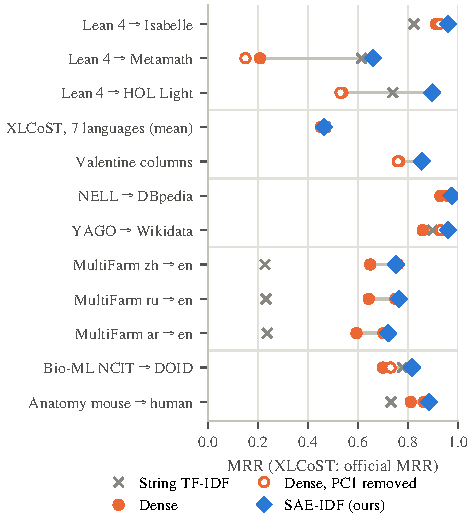
\includegraphics[width=0.55\textwidth]{figures/fig_main.pdf}
  \caption{Main-table results as MRR (Valentine: MRR; XLCoST: official MRR averaged over languages). The grey bar joins Dense to \method. \method beats Dense on every task, and the gap is widest where the two notations share the least surface form.}
  \label{fig:main}
\end{figure}

\begin{table}[H]
  \centering\footnotesize
  \begin{tabular}{@{}lrrrrrr@{}}
\toprule
Task & Queries & Strings & Dense & $-$PC1 & SAE unw. & \textbf{SAE-IDF} \\
\midrule
Bio-ML NCIT $\to$ DOID, valid split & 634 & 0.779 & 0.701 & 0.732 & 0.696 & \textbf{0.817} \\
Bio-ML NCIT $\to$ DOID, train split & 3,845 & 0.789 & 0.736 & 0.758 & 0.736 & \textbf{0.815} \\
OAEI Anatomy, mouse $\to$ human & 1,516 & 0.734 & 0.812 & 0.864 & 0.801 & \textbf{0.886} \\
\midrule
PubChem SMILES $\to$ IUPAC & 1,000 & 0.009 & 0.027 & 0.012 & 0.026 & 0.015 \\
PubChem SMILES $\to$ InChI & 1,000 & 0.008 & 0.007 & 0.009 & 0.005 & 0.029 \\
PubChem IUPAC $\to$ InChI & 1,000 & 0.012 & 0.006 & 0.008 & 0.005 & 0.020 \\
\bottomrule
\end{tabular}

  \caption{Appendix tasks with native context (MRR). Bio-ML uses its 100-candidate ranking protocol; Anatomy ranks all 3,298 human classes. PubChem's chance level is 0.0075 and no method exceeds 0.03.}
  \label{tab:apptasks}
\end{table}

\section{Embedding-model baseline}
\label{app:embed}

BGE-M3 \citep{chen2024bge} (XLM-RoBERTa-large, CLS pooling, inputs truncated to 1,024 tokens as for the LLM) embeds exactly the view texts used elsewhere: the statement or program, the whole-column text for Valentine, and each native view for classes and terms, averaged per symbol.
Candidates and metrics are those of the main table; the centred and PC1-removed variants use the same reference collections as for the LLM hidden state (Table~\ref{tab:embed}).

\begin{table}[H]
  \centering\scriptsize
  \begin{tabular}{@{}llrrrrrr@{}}
\toprule
 & & & \multicolumn{2}{c}{Gemma-2-9B} & \multicolumn{3}{c}{BGE-M3 embeddings} \\
\cmidrule(lr){4-5}\cmidrule(lr){6-8}
Task & Metric & Strings & Dense & \textbf{SAE-IDF} & plain & centred & $-$PC1 \\
\midrule
Lean 4 $\to$ Isabelle & MRR & 0.825 & 0.912 & \textbf{0.961} & 0.956 & 0.954 & 0.932 \\
Lean 4 $\to$ Metamath & MRR & 0.615 & 0.210 & 0.661 & \textbf{0.819} & 0.591 & 0.583 \\
Lean 4 $\to$ HOL Light & MRR & 0.741 & 0.539 & 0.898 & 0.967 & 0.967 & \textbf{0.967} \\
XLCoST, 7 languages & MRR & 0.468 & 0.454 & \textbf{0.464} & 0.438 & 0.437 & 0.451 \\
XLCoST, 7 languages & P@6 & 0.745 & 0.680 & \textbf{0.732} & 0.671 & 0.669 & 0.702 \\
Valentine columns & F1 & -- & 0.533 & 0.614 & \textbf{0.645} & 0.638 & 0.612 \\
Valentine columns & MRR & -- & 0.766 & 0.856 & 0.879 & \textbf{0.890} & 0.875 \\
NELL $\to$ DBpedia & MRR & 0.936 & 0.931 & 0.976 & 0.983 & \textbf{0.988} & 0.984 \\
YAGO $\to$ Wikidata & MRR & 0.899 & 0.860 & \textbf{0.962} & 0.910 & 0.925 & 0.958 \\
MultiFarm zh $\to$ en & MRR & 0.230 & 0.650 & \textbf{0.754} & 0.716 & 0.715 & 0.743 \\
MultiFarm ru $\to$ en & MRR & 0.234 & 0.644 & \textbf{0.765} & 0.718 & 0.715 & 0.726 \\
MultiFarm ar $\to$ en & MRR & 0.238 & 0.595 & \textbf{0.722} & 0.670 & 0.681 & 0.701 \\
Bio-ML valid & MRR & 0.779 & 0.701 & \textbf{0.817} & 0.611 & 0.617 & 0.611 \\
Bio-ML train & MRR & 0.789 & 0.736 & \textbf{0.815} & 0.636 & 0.644 & 0.740 \\
Anatomy & MRR & 0.734 & 0.812 & \textbf{0.886} & 0.789 & 0.810 & 0.853 \\
\bottomrule
\end{tabular}

  \caption{An off-the-shelf retriever against \method. Bold: best of the five model-based columns. The retriever leads on Lean~4 $\to$ Metamath, $\to$ HOL Light, Valentine and NELL $\to$ DBpedia; \method leads on the other main-table rows and on the three biomedical appendix tasks.}
  \label{tab:embed}
\end{table}

\section{XLCoST without the free hit}
\label{app:exclude}

The official XLCoST pool contains the query's own row, which every method retrieves first.
Table~\ref{tab:exclude} removes it, so the metrics count only the other-language versions of each program.

\begin{table}[H]
  \centering\footnotesize
  \begin{tabular}{@{}lrlrrrrr@{}}
\toprule
Query language & Programs & Metric & Strings & Dense & $-$PC1 & SAE unw. & \textbf{SAE-IDF} \\
\midrule
Java & 3,918 & MRR & \textbf{0.558} & 0.528 & 0.527 & 0.516 & 0.551 \\
 &  & P@6 & \textbf{0.550} & 0.459 & 0.458 & 0.445 & 0.534 \\
C++ & 3,895 & MRR & \textbf{0.560} & 0.536 & 0.535 & 0.530 & 0.549 \\
 &  & P@6 & \textbf{0.554} & 0.496 & 0.493 & 0.494 & 0.531 \\
Python & 3,853 & MRR & 0.560 & 0.545 & 0.536 & 0.540 & \textbf{0.561} \\
 &  & P@6 & \textbf{0.557} & 0.540 & 0.528 & 0.526 & 0.553 \\
C\# & 3,898 & MRR & \textbf{0.561} & 0.530 & 0.530 & 0.522 & 0.553 \\
 &  & P@6 & \textbf{0.552} & 0.467 & 0.469 & 0.472 & 0.538 \\
JavaScript & 3,851 & MRR & \textbf{0.563} & 0.547 & 0.542 & 0.538 & 0.557 \\
 &  & P@6 & \textbf{0.558} & 0.528 & 0.522 & 0.519 & 0.545 \\
PHP & 1,566 & MRR & 0.500 & 0.488 & 0.488 & 0.487 & \textbf{0.502} \\
 &  & P@6 & 0.658 & 0.633 & 0.637 & 0.626 & \textbf{0.661} \\
C & 283 & MRR & \textbf{0.457} & 0.435 & 0.438 & 0.438 & 0.452 \\
 &  & P@6 & 0.712 & 0.699 & 0.709 & 0.695 & \textbf{0.730} \\
\bottomrule
\end{tabular}

  \caption{XLCoST program-level search with the query's own row excluded from the pool (official metric definitions otherwise). \method beats Dense in every language on both metrics; word TF-IDF stays marginally ahead on MRR in most languages.}
  \label{tab:exclude}
\end{table}

\section{Generated contexts}
\label{app:generated}

\begin{table}[H]
  \centering\footnotesize
  \begin{tabular}{@{}llrrrrr@{}}
\toprule
Task & Contexts & Strings & Dense & $-$PC1 & SAE unw. & \textbf{SAE-IDF} \\
\midrule
NELL $\to$ DBpedia & two LLMs & 0.936 & 0.964 & 0.966 & 0.916 & \textbf{0.969} \\
 & one LLM & 0.936 & 0.927 & \textbf{0.972} & 0.904 & 0.972 \\
 & native & 0.936 & 0.931 & 0.957 & 0.938 & \textbf{0.976} \\
\addlinespace[2pt]
YAGO $\to$ Wikidata & two LLMs & 0.899 & 0.908 & \textbf{0.977} & 0.915 & 0.973 \\
 & one LLM & 0.899 & 0.917 & \textbf{0.968} & 0.920 & 0.968 \\
 & native & 0.899 & 0.860 & 0.932 & 0.872 & \textbf{0.962} \\
\addlinespace[2pt]
MultiFarm zh $\to$ en & two LLMs & 0.067 & 0.780 & \textbf{0.825} & 0.492 & 0.819 \\
 & one LLM & 0.067 & 0.753 & \textbf{0.787} & 0.478 & 0.786 \\
 & native & 0.230 & 0.650 & \textbf{0.760} & 0.404 & 0.754 \\
\addlinespace[2pt]
MultiFarm ru $\to$ en & two LLMs & 0.067 & 0.703 & \textbf{0.840} & 0.270 & 0.811 \\
 & one LLM & 0.073 & 0.680 & \textbf{0.847} & 0.248 & 0.807 \\
 & native & 0.234 & 0.644 & 0.751 & 0.252 & \textbf{0.765} \\
\addlinespace[2pt]
MultiFarm ar $\to$ en & two LLMs & 0.066 & 0.588 & \textbf{0.773} & 0.195 & 0.753 \\
 & one LLM & 0.066 & 0.595 & \textbf{0.794} & 0.163 & 0.724 \\
 & native & 0.238 & 0.595 & 0.702 & 0.225 & \textbf{0.722} \\
\addlinespace[2pt]
Drug brand $\to$ generic & two LLMs & \textbf{0.762} & 0.401 & 0.464 & 0.276 & 0.448 \\
 & one LLM, shared metadata & \textbf{0.828} & 0.384 & 0.456 & 0.277 & 0.441 \\
\addlinespace[2pt]
\bottomrule
\end{tabular}

  \caption{Generated versus native contexts (MRR). ``One LLM'': both sides described by the same generator; ``two LLMs'': the source side by one generator and the target side by another, each seeing only its own system's data; ``shared metadata'': the first drug run, in which both names were given the same pharmacologic-class text. With generated text, removing the first principal component of the dense vectors matches or beats \method; with native context it does not. Drug names have no native context and are not in the main table.}
  \label{tab:generated}
\end{table}

\section{Full ablation}
\label{app:ablation}

\begin{table}[H]
  \centering\small
  \begin{minipage}{0.92\textwidth}\begin{tabular}{@{}p{0.34\linewidth}p{0.3\linewidth}p{0.3\linewidth}@{}}
\toprule
Setting (Gemma-2-9B, layer 20, unless noted) & HOL Light & Metamath \\
\midrule
Dense baseline & 0.541 & 0.207 \\
\addlinespace[2pt]
\multicolumn{3}{@{}p{\linewidth}@{}}{\textit{SAE width} 16k / 32k / 65k / 131k / 262k / 524k / 1M, each at its canonical $L_0$ (68 / 57 / 55 / 114 / 50 / 48 / 101)} \\
\quad SAE-IDF & 0.82 / 0.86 / 0.89 / 0.90 / 0.91 / 0.93 / 0.93 & 0.62 / 0.61 / 0.71 / 0.67 / 0.68 / 0.70 / 0.66 \\
\addlinespace[2pt]
\multicolumn{3}{@{}p{\linewidth}@{}}{\textit{Sparsity}, average $L_0$ 11 / 19 / 34 / 53 / 62 / 114 / 221 / 276 (131k features)} \\
\quad SAE-IDF & 0.89 / 0.89 / 0.90 / 0.91 / 0.90 / 0.90 / 0.90 / 0.90 & 0.68 / 0.67 / 0.70 / 0.71 / 0.72 / 0.67 / 0.62 / 0.64 \\
\addlinespace[2pt]
\multicolumn{3}{@{}p{\linewidth}@{}}{\textit{Smaller model}: Gemma-2-2B, layer 12, width 16k / 65k / 262k} \\
\quad Dense & 0.462 & 0.257 \\
\quad SAE-IDF & 0.80 / 0.86 / 0.87 & 0.65 / 0.52 / 0.45 \\
\addlinespace[2pt]
\multicolumn{3}{@{}p{\linewidth}@{}}{\textit{Larger model}: Gemma-2-27B, layer 10 / 22 / 34 (131k, canonical $L_0$ 106 / 82 / 72)} \\
\quad Dense & 0.32 / 0.41 / 0.41 & 0.08 / 0.20 / 0.15 \\
\quad SAE-IDF & 0.84 / 0.94 / 0.58 & 0.41 / 0.74 / 0.60 \\
\bottomrule
\end{tabular}
\end{minipage}
  \caption{\method MRR across SAE width, sparsity and model size (Gemma Scope SAEs on Gemma-2-2B, 9B and 27B; miniF2F). Every entry beats the dense baseline in its row group.}
  \label{tab:ablation}
\end{table}

\begin{table}[H]
  \centering\small
  \begin{tabular}{@{}lrrrrrrrr@{}}
\toprule
 & \multicolumn{4}{c}{Lean 4 $\to$ HOL Light} & \multicolumn{4}{c}{Lean 4 $\to$ Metamath} \\
\cmidrule(lr){2-5}\cmidrule(lr){6-9}
Llama Scope SAE & Dense & PC1 rm. & SAE unw. & \textbf{SAE-IDF} & Dense & PC1 rm. & SAE unw. & \textbf{SAE-IDF} \\
\midrule
Layer 8, 131k & 0.502 & 0.587 & 0.436 & \textbf{0.743} & 0.500 & 0.516 & 0.567 & \textbf{0.674} \\
Layer 12, 131k & 0.509 & 0.614 & 0.451 & \textbf{0.815} & 0.630 & 0.624 & 0.582 & \textbf{0.711} \\
Layer 15, 131k & 0.603 & 0.699 & 0.611 & \textbf{0.906} & 0.646 & 0.637 & 0.675 & \textbf{0.787} \\
Layer 20, 131k & 0.304 & 0.290 & 0.209 & \textbf{0.666} & 0.269 & 0.343 & 0.369 & \textbf{0.719} \\
Layer 24, 131k & 0.291 & 0.267 & 0.274 & \textbf{0.751} & 0.124 & 0.273 & 0.202 & \textbf{0.661} \\
Layer 15, 32k & 0.603 & 0.699 & 0.583 & \textbf{0.845} & 0.646 & 0.637 & 0.626 & \textbf{0.741} \\
\bottomrule
\end{tabular}

  \caption{Second model family: Llama-3.1-8B with Llama Scope SAEs (MRR). \method beats Dense and \pcone in all six configurations on both tasks.}
  \label{tab:llama}
\end{table}

\paragraph{Beyond formal mathematics.}
Figure~\ref{fig:sweepkg} repeats the layer and width sweeps on Common-KG and MultiFarm with the same SAE files (the 262k and matched-sparsity 16k/1M files were not available on the cluster used for these runs).
Over the 45 (task, setting) pairs \method beats dense by +0.006 to +0.28 MRR and the unweighted code in every pair; \pcone is behind in 32 of 45 (15 of 15 on NELL $\to$ DBpedia, 10 on YAGO $\to$ Wikidata, 7 on MultiFarm).
On the knowledge-graph tasks every layer from 5 to 25 is within 0.03 MRR; on MultiFarm layers 15--25 are best; the last layers fall off everywhere.
Width helps less than on HOL Light: NELL $\to$ DBpedia rises slightly (0.964 to 0.979), YAGO $\to$ Wikidata is flat, and MultiFarm peaks at 65k features (0.774) and declines to 0.730 at 1M, while the unweighted code collapses as the dictionary widens (0.42 to 0.14).

\begin{figure}[H]
  \centering
  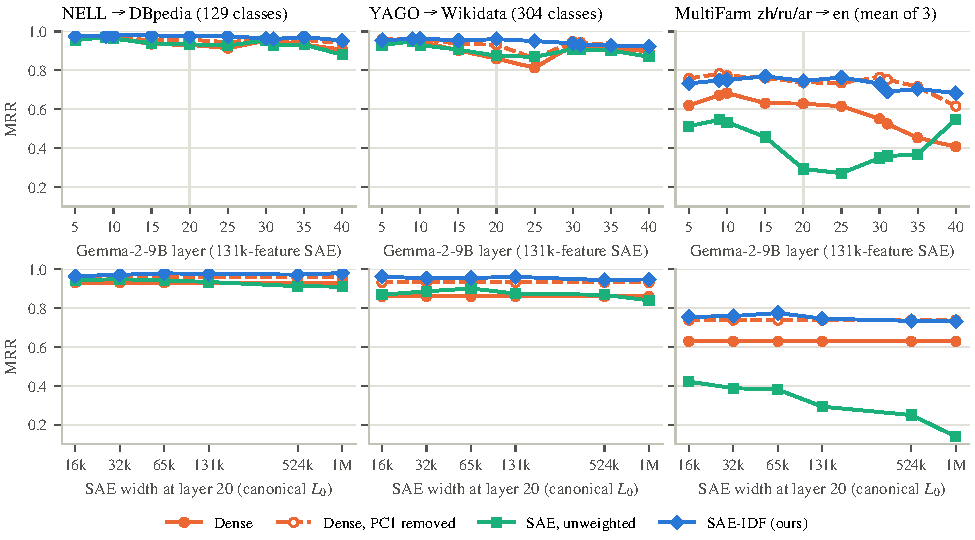
\includegraphics[width=0.95\textwidth]{figures/fig_sweep_kg.pdf}
  \caption{Layer sweep (top) and SAE-width sweep (bottom) on Common-KG and MultiFarm with native views, Gemma-2-9B. \method beats Dense and the unweighted code in every setting; \pcone is close on YAGO and MultiFarm.}
  \label{fig:sweepkg}
\end{figure}

\paragraph{Feature weightings.}
Every evaluator also scores the alternatives to collection idf that the pipeline computes: an idf from Neuronpedia's Pile activation densities (which needs no matched collection), an information weighting (log of in-symbol over background firing rate) and a log-odds weighting.
Collection idf is best on 10 of 13 comparisons (Table~\ref{tab:weightings}); the information weighting is close on ontology terms and tables, and the Pile-density idf is far behind on formal mathematics (0.190 vs.\ 0.661 on Metamath), where the generic features are specific to the pair of systems rather than to the Pile.

\begin{table}[H]
  \centering\footnotesize
  \begin{tabular}{@{}llrrrrr@{}}
\toprule
Task & Metric & Unweighted & \textbf{idf (collection)} & idf (Pile density) & Information & Log-odds \\
\midrule
Lean 4 $\to$ Isabelle & MRR & 0.882 & \textbf{0.961} & 0.908 & 0.740 & 0.756 \\
Lean 4 $\to$ Metamath & MRR & 0.095 & \textbf{0.661} & 0.190 & 0.102 & 0.190 \\
Lean 4 $\to$ HOL Light & MRR & 0.493 & \textbf{0.898} & 0.588 & 0.194 & 0.277 \\
XLCoST, 7 languages & MRR & 0.449 & 0.464 & 0.451 & 0.438 & \textbf{0.471} \\
Valentine columns & F1 & 0.458 & 0.614 & 0.574 & \textbf{0.615} & 0.592 \\
Valentine columns & MRR & 0.685 & \textbf{0.856} & 0.808 & 0.855 & 0.781 \\
NELL $\to$ DBpedia & MRR & 0.938 & \textbf{0.976} & 0.966 & 0.968 & 0.934 \\
YAGO $\to$ Wikidata & MRR & 0.872 & \textbf{0.962} & 0.941 & 0.947 & 0.914 \\
MultiFarm zh $\to$ en & MRR & 0.404 & \textbf{0.754} & 0.710 & 0.726 & 0.509 \\
MultiFarm ru $\to$ en & MRR & 0.252 & 0.765 & 0.699 & \textbf{0.765} & 0.319 \\
MultiFarm ar $\to$ en & MRR & 0.225 & \textbf{0.722} & 0.679 & 0.714 & 0.296 \\
Bio-ML valid & MRR & 0.696 & \textbf{0.817} & 0.793 & 0.811 & 0.760 \\
Anatomy & MRR & 0.801 & \textbf{0.886} & 0.863 & 0.885 & 0.846 \\
\bottomrule
\end{tabular}

  \caption{Alternative feature weightings on the same sparse codes (MRR unless stated). Bold: best per row.}
  \label{tab:weightings}
\end{table}

\paragraph{Four-prover merge.}
Running all twelve ordered pairs among Lean~4, Isabelle, Metamath and HOL Light (Gemma-2-9B, layer 20) and merging mutual-top-1 matches as for XLCoST gives Table~\ref{tab:provermerge}: \method's alignments are more precise, cover almost twice as many statements, and compose into fewer, purer components.

\begin{table}[H]
  \centering\footnotesize
  \begin{tabular}{@{}lrrrrr@{}}
\toprule
Method & Mutual-top-1 precision & Coverage & Transitivity & Merge purity & ARI \\
\midrule
Dense & 0.900 & 0.340 & 0.963 & 0.979 & 0.519 \\
Dense$_{-\mathrm{PC1}}$ & 0.900 & 0.340 & 0.963 & 0.979 & 0.519 \\
SAE unweighted & 0.616 & 0.299 & 0.902 & 0.958 & 0.432 \\
\textbf{SAE-IDF} & 0.983 & 0.639 & 0.981 & 0.981 & 0.795 \\
\bottomrule
\end{tabular}

  \caption{Merge and transitivity over the four miniF2F provers (489 problems, up to four statements each). Precision and coverage are means over the twelve ordered pairs' mutual-top-1 alignments.}
  \label{tab:provermerge}
\end{table}

\paragraph{Second model family on the whole main table.}
Table~\ref{tab:llamamain} runs Llama-3.1-8B with the Llama Scope layer-15 131k SAE on every main-table task with the same native views.
\method beats dense on 11 of the 12 rows and \pcone on 9: the formal-mathematics gains carry over (Llama's dense state is far stronger on Metamath), Valentine improves (F1 0.625 vs.\ 0.588 dense, MRR 0.862), the knowledge-graph and cross-lingual tasks are ties or small deficits against \pcone (NELL $\to$ DBpedia 0.958 vs.\ 0.960, MultiFarm ru $\to$ en 0.726 vs.\ 0.751), and on XLCoST \method trails dense by 0.01 MRR while leading on Precision@6.
On the appendix tasks it leads on Bio-ML and trails \pcone on Anatomy.

\begin{table}[H]
  \centering\footnotesize
  \setlength{\tabcolsep}{4pt}
  \begin{tabular}{@{}llrrrrrrrr@{}}
\toprule
 & & & \multicolumn{2}{c}{Gemma-2-9B, L20} & \multicolumn{4}{c}{Llama-3.1-8B, L15} \\
\cmidrule(lr){4-5}\cmidrule(lr){6-9}
Task & Metric & Strings & Dense & \textbf{SAE-IDF} & Dense & $-$PC1 & SAE unw. & \textbf{SAE-IDF} \\
\midrule
Lean 4 $\to$ Isabelle & MRR & 0.825 & 0.912 & 0.961 & 0.942 & 0.944 & 0.942 & \textbf{0.976} \\
Lean 4 $\to$ Metamath & MRR & 0.615 & 0.210 & 0.661 & 0.646 & 0.637 & 0.675 & \textbf{0.787} \\
Lean 4 $\to$ HOL Light & MRR & 0.741 & 0.539 & 0.898 & 0.603 & 0.699 & 0.611 & \textbf{0.906} \\
XLCoST, 7 languages & MRR & 0.468 & 0.454 & 0.464 & \textbf{0.451} & 0.447 & 0.448 & 0.442 \\
XLCoST, 7 languages & P@6 & 0.745 & 0.680 & 0.732 & 0.641 & 0.648 & 0.634 & \textbf{0.657} \\
Valentine columns & F1 & -- & 0.533 & 0.614 & 0.588 & 0.579 & 0.592 & \textbf{0.625} \\
Valentine columns & MRR & -- & 0.766 & 0.856 & 0.786 & 0.811 & 0.760 & \textbf{0.862} \\
NELL $\to$ DBpedia & MRR & 0.936 & 0.931 & 0.976 & 0.949 & \textbf{0.960} & 0.930 & 0.958 \\
YAGO $\to$ Wikidata & MRR & 0.899 & 0.860 & 0.962 & 0.889 & 0.944 & 0.915 & \textbf{0.944} \\
MultiFarm zh $\to$ en & MRR & 0.230 & 0.650 & 0.754 & 0.659 & 0.779 & 0.585 & \textbf{0.787} \\
MultiFarm ru $\to$ en & MRR & 0.234 & 0.644 & 0.765 & 0.661 & \textbf{0.751} & 0.616 & 0.726 \\
MultiFarm ar $\to$ en & MRR & 0.238 & 0.595 & 0.722 & 0.578 & 0.669 & 0.468 & \textbf{0.672} \\
\midrule
Bio-ML valid (appendix task) & MRR & 0.779 & 0.701 & 0.817 & 0.704 & 0.710 & 0.723 & \textbf{0.779} \\
Bio-ML train (appendix task) & MRR & 0.789 & 0.736 & 0.815 & 0.727 & 0.743 & 0.749 & \textbf{0.789} \\
Anatomy (appendix task) & MRR & 0.734 & 0.812 & 0.886 & 0.800 & \textbf{0.871} & 0.823 & 0.844 \\
\bottomrule
\end{tabular}

  \caption{Main-table tasks with a second model family. Llama-3.1-8B, layer 15, Llama Scope 131k features, native views; Gemma-2-9B columns repeat Table~\ref{tab:main}. Bold: best of the four Llama methods.}
  \label{tab:llamamain}
\end{table}

\paragraph{Llama layers on knowledge-graph and cross-lingual terms.}
Table~\ref{tab:llamakg} repeats the Common-KG and MultiFarm runs with every Llama Scope layer: the layer-15 ties with \pcone become leads at layers 8 and 12 on both knowledge-graph pairs; on MultiFarm (mean of the three language pairs) \method leads at layers 12, 20 and 24 and trails \pcone by at most 0.012 at the others. Across the 18 (task, layer) cells \method beats dense in 16 and \pcone in 10.

\begin{table}[H]
  \centering\footnotesize
  \begin{tabular}{@{}llrrrr@{}}
\toprule
Task & Llama Scope SAE & Dense & $-$PC1 & SAE unw. & \textbf{SAE-IDF} \\
\midrule
NELL $\to$ DBpedia & layer 8, 131k & 0.953 & 0.960 & 0.945 & \textbf{0.970} \\
 & layer 12, 131k & 0.939 & 0.950 & 0.937 & \textbf{0.973} \\
 & layer 15, 131k & 0.949 & \textbf{0.960} & 0.930 & 0.958 \\
 & layer 15, 32k & 0.949 & 0.960 & 0.942 & \textbf{0.961} \\
 & layer 20, 131k & 0.947 & \textbf{0.958} & 0.904 & 0.947 \\
 & layer 24, 131k & 0.938 & \textbf{0.951} & 0.908 & 0.936 \\
YAGO $\to$ Wikidata & layer 8, 131k & 0.889 & 0.937 & 0.885 & \textbf{0.949} \\
 & layer 12, 131k & 0.806 & 0.922 & 0.861 & \textbf{0.955} \\
 & layer 15, 131k & 0.889 & 0.944 & 0.915 & \textbf{0.944} \\
 & layer 15, 32k & 0.889 & 0.944 & 0.920 & \textbf{0.955} \\
 & layer 20, 131k & 0.912 & \textbf{0.935} & 0.899 & 0.928 \\
 & layer 24, 131k & 0.915 & \textbf{0.936} & 0.875 & 0.926 \\
MultiFarm & layer 8, 131k & 0.672 & \textbf{0.751} & 0.575 & 0.739 \\
 & layer 12, 131k & 0.583 & 0.687 & 0.496 & \textbf{0.758} \\
 & layer 15, 131k & 0.633 & \textbf{0.733} & 0.556 & 0.728 \\
 & layer 15, 32k & 0.633 & \textbf{0.733} & 0.528 & 0.726 \\
 & layer 20, 131k & 0.625 & 0.716 & 0.470 & \textbf{0.722} \\
 & layer 24, 131k & 0.523 & 0.684 & 0.307 & \textbf{0.704} \\
\bottomrule
\end{tabular}

  \caption{Llama-3.1-8B layer sweep on Common-KG and MultiFarm (mean of the three pairs), native views, MRR.}
  \label{tab:llamakg}
\end{table}

\paragraph{Seed study.}
The only stochastic step is the sampling of views: up to 16 instances per Common-KG class and 16 cell values per Valentine column.
Table~\ref{tab:seeds} repeats the main-table runs with other sampling seeds (four seeds for Common-KG, three for Valentine); the ranges are far smaller than the gaps between methods.

\begin{table}[H]
  \centering\footnotesize
  \begin{tabular}{@{}lrrrrr@{}}
\toprule
Task & Seeds & Dense & $-$PC1 & SAE unw. & \textbf{SAE-IDF} \\
\midrule
NELL $\to$ DBpedia & 4 & 0.934 $\pm$ 0.002 & 0.954 $\pm$ 0.003 & 0.933 $\pm$ 0.004 & 0.976 $\pm$ 0.000 \\
YAGO $\to$ Wikidata & 4 & 0.861 $\pm$ 0.001 & 0.932 $\pm$ 0.003 & 0.874 $\pm$ 0.002 & 0.960 $\pm$ 0.002 \\
Valentine (F1) & 3 & 0.535 $\pm$ 0.002 & 0.534 $\pm$ 0.003 & 0.459 $\pm$ 0.002 & 0.614 $\pm$ 0.001 \\
Valentine (MRR) & 3 & 0.768 $\pm$ 0.001 & 0.762 $\pm$ 0.001 & 0.685 $\pm$ 0.002 & 0.857 $\pm$ 0.002 \\
\bottomrule
\end{tabular}

  \caption{Mean $\pm$ half-range over sampling seeds (MRR unless stated). Gemma-2-9B, layer 20, 131k SAE.}
  \label{tab:seeds}
\end{table}

\begin{table}[H]
  \centering\footnotesize
  \setlength{\tabcolsep}{4pt}
  \begin{tabular}{@{}lrrrrrrrr@{}}
\toprule
 & \multicolumn{4}{c}{Lean 4 $\to$ HOL Light} & \multicolumn{4}{c}{Lean 4 $\to$ Metamath} \\
\cmidrule(lr){2-5}\cmidrule(lr){6-9}
Configuration & Dense & PC1 rm. & SAE unw. & \textbf{SAE-IDF} & Dense & PC1 rm. & SAE unw. & \textbf{SAE-IDF} \\
\midrule
Gemma-2-9B, layer 5, 131k & 0.248 & 0.224 & 0.177 & \textbf{0.800} & 0.138 & 0.159 & 0.068 & \textbf{0.512} \\
layer 9 & 0.317 & 0.320 & 0.348 & \textbf{0.840} & 0.190 & 0.172 & 0.140 & \textbf{0.583} \\
layer 10 & 0.335 & 0.330 & 0.433 & \textbf{0.867} & 0.212 & 0.175 & 0.130 & \textbf{0.451} \\
layer 15 & 0.458 & 0.434 & 0.524 & \textbf{0.880} & 0.233 & 0.173 & 0.100 & \textbf{0.727} \\
layer 20 ($L_0$ 114, main table) & 0.541 & 0.530 & 0.493 & \textbf{0.900} & 0.207 & 0.149 & 0.092 & \textbf{0.667} \\
layer 25 & 0.439 & 0.553 & 0.280 & \textbf{0.882} & 0.179 & 0.145 & 0.112 & \textbf{0.623} \\
layer 30 & 0.214 & 0.248 & 0.144 & \textbf{0.739} & 0.123 & 0.089 & 0.088 & \textbf{0.693} \\
layer 31 & 0.210 & 0.209 & 0.122 & \textbf{0.757} & 0.121 & 0.076 & 0.077 & \textbf{0.703} \\
layer 35 & 0.225 & 0.204 & 0.115 & \textbf{0.716} & 0.100 & 0.076 & 0.078 & \textbf{0.594} \\
layer 40 & 0.173 & 0.139 & 0.080 & \textbf{0.464} & 0.077 & 0.049 & 0.039 & \textbf{0.301} \\
layer 20, 16k ($L_0$ 68) & 0.541 & 0.530 & 0.521 & \textbf{0.820} & 0.207 & 0.149 & 0.119 & \textbf{0.625} \\
layer 20, 16k ($L_0$ 58) & 0.541 & 0.531 & 0.490 & \textbf{0.817} & 0.209 & 0.151 & 0.114 & \textbf{0.621} \\
layer 20, 32k ($L_0$ 57) & 0.541 & 0.530 & 0.503 & \textbf{0.862} & 0.207 & 0.149 & 0.109 & \textbf{0.608} \\
layer 20, 65k ($L_0$ 55) & 0.541 & 0.530 & 0.417 & \textbf{0.890} & 0.207 & 0.149 & 0.086 & \textbf{0.706} \\
layer 20, 262k ($L_0$ 50) & 0.541 & 0.531 & 0.442 & \textbf{0.912} & 0.209 & 0.151 & 0.063 & \textbf{0.684} \\
layer 20, 524k ($L_0$ 48) & 0.541 & 0.530 & 0.462 & \textbf{0.927} & 0.207 & 0.149 & 0.060 & \textbf{0.698} \\
layer 20, 1M ($L_0$ 101) & 0.541 & 0.530 & 0.455 & \textbf{0.931} & 0.207 & 0.149 & 0.077 & \textbf{0.659} \\
layer 20, 1M ($L_0$ 57) & 0.541 & 0.531 & 0.436 & \textbf{0.935} & 0.209 & 0.151 & 0.059 & \textbf{0.668} \\
layer 20, 131k, $L_0$ 11 & 0.541 & 0.530 & 0.403 & \textbf{0.894} & 0.207 & 0.149 & 0.046 & \textbf{0.676} \\
$L_0$ 19 & 0.541 & 0.530 & 0.314 & \textbf{0.893} & 0.207 & 0.149 & 0.056 & \textbf{0.670} \\
$L_0$ 34 & 0.541 & 0.530 & 0.423 & \textbf{0.904} & 0.207 & 0.149 & 0.057 & \textbf{0.700} \\
$L_0$ 53 & 0.541 & 0.530 & 0.462 & \textbf{0.906} & 0.207 & 0.149 & 0.080 & \textbf{0.708} \\
$L_0$ 62 & 0.541 & 0.530 & 0.517 & \textbf{0.904} & 0.207 & 0.149 & 0.084 & \textbf{0.720} \\
$L_0$ 221 & 0.541 & 0.530 & 0.501 & \textbf{0.896} & 0.207 & 0.149 & 0.109 & \textbf{0.625} \\
$L_0$ 276 & 0.541 & 0.530 & 0.487 & \textbf{0.897} & 0.207 & 0.149 & 0.116 & \textbf{0.639} \\
Gemma-2-2B, layer 12, 16k & 0.462 & 0.487 & 0.492 & \textbf{0.800} & 0.257 & 0.238 & 0.236 & \textbf{0.651} \\
Gemma-2-2B, layer 12, 65k & 0.462 & 0.487 & 0.575 & \textbf{0.862} & 0.257 & 0.238 & 0.122 & \textbf{0.523} \\
Gemma-2-2B, layer 12, 262k & 0.462 & 0.487 & 0.491 & \textbf{0.872} & 0.257 & 0.238 & 0.156 & \textbf{0.452} \\
Llama-3.1-8B, layer 8, 131k & 0.502 & 0.587 & 0.436 & \textbf{0.743} & 0.500 & 0.516 & 0.567 & \textbf{0.674} \\
Llama-3.1-8B, layer 12, 131k & 0.509 & 0.614 & 0.451 & \textbf{0.815} & 0.630 & 0.624 & 0.582 & \textbf{0.711} \\
Llama-3.1-8B, layer 15, 131k & 0.603 & 0.699 & 0.611 & \textbf{0.906} & 0.646 & 0.637 & 0.675 & \textbf{0.787} \\
Llama-3.1-8B, layer 15, 32k & 0.603 & 0.699 & 0.583 & \textbf{0.845} & 0.646 & 0.637 & 0.626 & \textbf{0.741} \\
Llama-3.1-8B, layer 20, 131k & 0.304 & 0.290 & 0.209 & \textbf{0.666} & 0.269 & 0.343 & 0.369 & \textbf{0.719} \\
Llama-3.1-8B, layer 24, 131k & 0.291 & 0.267 & 0.274 & \textbf{0.751} & 0.124 & 0.273 & 0.202 & \textbf{0.661} \\
Gemma-2-27B, layer 10, 131k ($L_0$ 106) & 0.319 & 0.288 & 0.282 & \textbf{0.843} & 0.077 & 0.114 & 0.058 & \textbf{0.405} \\
Gemma-2-27B, layer 22, 131k ($L_0$ 82) & 0.408 & 0.328 & 0.282 & \textbf{0.939} & 0.199 & 0.097 & 0.139 & \textbf{0.738} \\
Gemma-2-27B, layer 22, 131k ($L_0$ 48) & 0.408 & 0.328 & 0.281 & \textbf{0.917} & 0.199 & 0.097 & 0.126 & \textbf{0.731} \\
Gemma-2-27B, layer 22, 131k ($L_0$ 150) & 0.408 & 0.328 & 0.280 & \textbf{0.924} & 0.199 & 0.097 & 0.172 & \textbf{0.709} \\
Gemma-2-27B, layer 34, 131k ($L_0$ 72) & 0.407 & 0.491 & 0.154 & \textbf{0.584} & 0.145 & 0.126 & 0.083 & \textbf{0.597} \\
\bottomrule
\end{tabular}

  \caption{All 39 ablation configurations (78 runs) on miniF2F Lean~4 $\to$ HOL Light and $\to$ Metamath (MRR). Gemma Scope widths are given at the sparsity used; ``$L_0$'' rows are the 131k-feature SAE at layer 20. \method beats Dense, \pcone and \saemean in every run.}
  \label{tab:ablationfull}
\end{table}

\section{Feature-level decomposition and case studies}
\label{app:cases}

\begin{figure}[H]
  \centering
  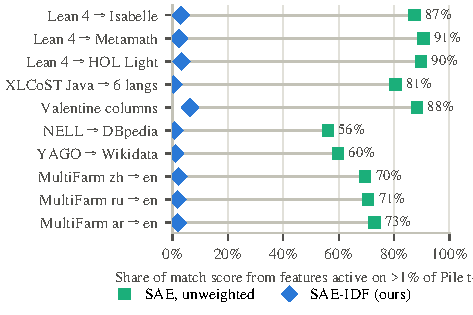
\includegraphics[width=0.55\textwidth]{figures/fig_interp.pdf}
  \caption{Share of each correct match's cosine carried by features that fire on more than 1\% of Pile tokens. Without weighting (squares) these ubiquitous features carry 56--91\% of the evidence on every task; with rarity weighting (diamonds) they carry 0--6\%.}
  \label{fig:interp}
\end{figure}

\begin{table}[H]
  \centering\scriptsize
  \begin{tabular}{@{}lrrrrr@{}}
\toprule
Task & Matches & \makecell[r]{Common ($>$1\%):\\unw. $\to$ SAE-IDF} & \makecell[r]{Rare ($<$0.1\%)\\SAE-IDF} & \makecell[r]{Features for\\50\% / 80\%} & \makecell[r]{Concept / surface / notation\\(SAE-IDF top-5)} \\
\midrule
Lean 4 $\to$ Isabelle & 300 & 87\% $\to$ 3\% & 32\% & 21 / 146 & 43\% / 7\% / 48\% \\
Lean 4 $\to$ Metamath & 259 & 91\% $\to$ 2\% & 31\% & 15 / 88 & 39\% / 4\% / 55\% \\
Lean 4 $\to$ HOL Light & 271 & 90\% $\to$ 3\% & 30\% & 17 / 137 & 46\% / 8\% / 44\% \\
XLCoST, Java $\to$ 6 languages & 300 & 81\% $\to$ 0\% & 75\% & 10 / 88 & 51\% / 11\% / 35\% \\
Valentine columns & 300 & 88\% $\to$ 6\% & 49\% & 10 / 54 & 79\% / 4\% / 13\% \\
NELL $\to$ DBpedia & 124 & 56\% $\to$ 1\% & 94\% & 1 / 2 & 94\% / 5\% / 1\% \\
YAGO $\to$ Wikidata & 286 & 60\% $\to$ 1\% & 93\% & 1 / 3 & 87\% / 11\% / 2\% \\
MultiFarm zh $\to$ en & 162 & 70\% $\to$ 2\% & 87\% & 1 / 4 & 69\% / 26\% / 1\% \\
MultiFarm ru $\to$ en & 163 & 71\% $\to$ 2\% & 88\% & 1 / 4 & 72\% / 24\% / 2\% \\
MultiFarm ar $\to$ en & 150 & 73\% $\to$ 2\% & 87\% & 2 / 4 & 71\% / 24\% / 1\% \\
\bottomrule
\end{tabular}

  \caption{Feature-level decomposition of correct matches. \emph{Common}: share of the cosine from features active on $>$1\% of Pile tokens, under the unweighted code and under \method. \emph{Rare}: share from features active on $<$0.1\%. \emph{Features for 50\%/80\%}: median number of shared features needed to reach that share of the cosine. The last column splits \method's five largest contributions per match by explanation type.}
  \label{tab:interp}
\end{table}

Cases were selected per task by three rules, applied to the evaluation's own rankings: \emph{wins}, correct \method matches whose gold counterpart Dense ranks 5th or worse, taking the shortest query texts with the widest \method margin over the runner-up; \emph{failures}, pairs where Dense ranks the gold counterpart first and \method does not, taking the shortest; and the features carrying the most \method evidence over all decomposed matches of the task.
For each case we list the gold's rank under every method, the top five shared features with their share of the cosine and Pile density, the same pair's top shared features without weighting, and, for failures, the features shared with the wrong top candidate.
One XLCoST ``failure'' was excluded because the dataset contains the program twice.
The full listings for all ten tasks (31 cases) are released with the code.

\section{Abstention}
\label{app:abstention}

If a matcher may abstain, how much coverage does it keep at a given precision?
For every query the confidence is the cosine margin between the best and the second-best candidate; queries are answered in decreasing order of confidence.
Table~\ref{tab:abstention} gives top-1 accuracy with every query answered and the coverage at which precision first drops below 90\% and 95\%, for \method and the dense hidden state, from the same weights the evaluation used (XLCoST is omitted because its official pool contains the query's own row).

\begin{table}[H]
  \centering\footnotesize
  \begin{tabular}{@{}lrrrrrrr@{}}
\toprule
 & & \multicolumn{3}{c}{Dense} & \multicolumn{3}{c}{\textbf{SAE-IDF}} \\
\cmidrule(lr){3-5}\cmidrule(lr){6-8}
Task & $n$ & Top-1 & Cov.@90\% & Cov.@95\% & Top-1 & Cov.@90\% & Cov.@95\% \\
\midrule
Lean 4 $\to$ Isabelle & 483 & 0.880 & 0.96 & 0.89 & 0.936 & 1.00 & 0.98 \\
Lean 4 $\to$ Metamath & 482 & 0.127 & 0.01 & 0.01 & 0.537 & 0.24 & 0.21 \\
Lean 4 $\to$ HOL Light & 317 & 0.454 & 0.24 & 0.20 & 0.855 & 0.93 & 0.85 \\
Valentine columns & 8,346 & 0.622 & 0.38 & 0.22 & 0.738 & 0.67 & 0.53 \\
NELL $\to$ DBpedia & 129 & 0.899 & 0.99 & 0.91 & 0.961 & 1.00 & 1.00 \\
YAGO $\to$ Wikidata & 304 & 0.819 & 0.89 & 0.76 & 0.941 & 1.00 & 0.97 \\
MultiFarm zh $\to$ en & 246 & 0.549 & 0.42 & 0.32 & 0.659 & 0.41 & 0.30 \\
MultiFarm ru $\to$ en & 246 & 0.553 & 0.29 & 0.20 & 0.663 & 0.34 & 0.20 \\
MultiFarm ar $\to$ en & 239 & 0.523 & 0.31 & 0.21 & 0.628 & 0.44 & 0.24 \\
\bottomrule
\end{tabular}

  \caption{Margin-based abstention. Cov.@90\%: the fraction of queries that can be answered while top-1 precision stays at or above 90\%.}
  \label{tab:abstention}
\end{table}

\section{Statistical significance}
\label{app:significance}

For every comparison in the main table we take the per-query quantity that the metric averages (the official per-query MRR for miniF2F and XLCoST, the per-pair F1 or MRR for Valentine, the reciprocal rank of the gold counterpart for the ontology and knowledge-graph tasks), resample the queries with replacement 10,000 times, and report the mean difference \method minus baseline with its 95\% percentile interval and the one-sided bootstrap $p$-value $P(\Delta\le 0)$ (Table~\ref{tab:significance}).
Every gain over Dense has $p<0.004$.
The gain over \pcone has $p<0.01$ on 12 of 16 comparisons; on the three MultiFarm pairs and on NELL $\to$ DBpedia the interval covers zero.
Against strings, \method is significantly ahead on all formal-mathematics, knowledge-graph and ontology tasks (Lean~4 $\to$ Metamath marginally, $p=0.02$), tied on XLCoST Python, PHP and C, and significantly behind word TF-IDF on XLCoST Java, C++, C\# and JavaScript.
Table~\ref{tab:significancellama} repeats the analysis for the Llama-3.1-8B runs: the gains over dense stay significant on the formal-mathematics, Valentine, YAGO, MultiFarm and biomedical tasks, while NELL $\to$ DBpedia and the XLCoST languages are ties or small deficits, and \pcone is significantly ahead on Anatomy.

\begin{table}[H]
  \centering\scriptsize
  \setlength{\tabcolsep}{3.5pt}
  \begin{tabular}{@{}lrllllll@{}}
\toprule
 & & \multicolumn{2}{c}{vs.\ Dense} & \multicolumn{2}{c}{vs.\ Dense$_{-\mathrm{PC1}}$} & \multicolumn{2}{c}{vs.\ Strings} \\
\cmidrule(lr){3-4}\cmidrule(lr){5-6}\cmidrule(lr){7-8}
Task & $n$ & $\Delta$ [95\% CI] & $p$ & $\Delta$ [95\% CI] & $p$ & $\Delta$ [95\% CI] & $p$ \\
\midrule
Lean 4 $\to$ Isabelle & 483 & +0.048 [+0.027, +0.071] & $<$.001 & +0.034 [+0.014, +0.055] & $<$.001 & +0.136 [+0.105, +0.168] & $<$.001 \\
Lean 4 $\to$ Metamath & 482 & +0.451 [+0.418, +0.485] & $<$.001 & +0.510 [+0.475, +0.546] & $<$.001 & +0.046 [+0.002, +0.090] & 0.02 \\
Lean 4 $\to$ HOL Light & 317 & +0.359 [+0.315, +0.405] & $<$.001 & +0.367 [+0.322, +0.412] & $<$.001 & +0.157 [+0.114, +0.200] & $<$.001 \\
XLCoST Java & 3,918 & +0.014 [+0.013, +0.016] & $<$.001 & +0.015 [+0.013, +0.016] & $<$.001 & -0.005 [-0.006, -0.004] & 1.00 \\
XLCoST C++ & 3,895 & +0.008 [+0.007, +0.010] & $<$.001 & +0.009 [+0.008, +0.011] & $<$.001 & -0.008 [-0.009, -0.006] & 1.00 \\
XLCoST Python & 3,853 & +0.011 [+0.009, +0.012] & $<$.001 & +0.017 [+0.016, +0.019] & $<$.001 & +0.000 [-0.001, +0.002] & 0.25 \\
XLCoST C\# & 3,898 & +0.013 [+0.012, +0.015] & $<$.001 & +0.013 [+0.012, +0.015] & $<$.001 & -0.006 [-0.006, -0.005] & 1.00 \\
XLCoST JavaScript & 3,851 & +0.006 [+0.005, +0.008] & $<$.001 & +0.010 [+0.009, +0.012] & $<$.001 & -0.005 [-0.006, -0.004] & 1.00 \\
XLCoST PHP & 1,566 & +0.010 [+0.008, +0.011] & $<$.001 & +0.010 [+0.008, +0.011] & $<$.001 & +0.001 [-0.000, +0.003] & 0.07 \\
XLCoST C & 283 & +0.013 [+0.009, +0.016] & $<$.001 & +0.010 [+0.008, +0.013] & $<$.001 & -0.004 [-0.008, +0.000] & 0.96 \\
Valentine (F1) & 551 & +0.081 [+0.074, +0.089] & $<$.001 & +0.080 [+0.072, +0.089] & $<$.001 & -- \\
Valentine (MRR) & 551 & +0.090 [+0.075, +0.105] & $<$.001 & +0.095 [+0.082, +0.109] & $<$.001 & -- \\
NELL $\to$ DBpedia & 129 & +0.045 [+0.011, +0.081] & $<$.01 & +0.018 [-0.009, +0.048] & 0.11 & +0.040 [+0.014, +0.071] & $<$.001 \\
YAGO $\to$ Wikidata & 304 & +0.102 [+0.070, +0.136] & $<$.001 & +0.030 [+0.007, +0.054] & $<$.01 & +0.062 [+0.039, +0.087] & $<$.001 \\
MultiFarm zh $\to$ en & 246 & +0.104 [+0.058, +0.151] & $<$.001 & -0.006 [-0.040, +0.028] & 0.64 & +0.524 [+0.467, +0.578] & $<$.001 \\
MultiFarm ru $\to$ en & 246 & +0.121 [+0.079, +0.162] & $<$.001 & +0.014 [-0.017, +0.045] & 0.19 & +0.531 [+0.480, +0.581] & $<$.001 \\
MultiFarm ar $\to$ en & 239 & +0.127 [+0.088, +0.168] & $<$.001 & +0.019 [-0.016, +0.054] & 0.14 & +0.484 [+0.429, +0.539] & $<$.001 \\
Bio-ML valid & 634 & +0.117 [+0.094, +0.141] & $<$.001 & +0.086 [+0.064, +0.107] & $<$.001 & +0.038 [+0.017, +0.059] & $<$.001 \\
Bio-ML train & 3,845 & +0.080 [+0.071, +0.089] & $<$.001 & +0.057 [+0.049, +0.066] & $<$.001 & +0.026 [+0.019, +0.034] & $<$.001 \\
Anatomy & 1,516 & +0.074 [+0.061, +0.087] & $<$.001 & +0.021 [+0.009, +0.033] & $<$.001 & +0.152 [+0.137, +0.167] & $<$.001 \\
\bottomrule
\end{tabular}

  \caption{Paired bootstrap over queries (10,000 resamples): mean difference \method minus baseline, 95\% interval, and one-sided bootstrap $p$-value. Valentine has no string baseline.}
  \label{tab:significance}
\end{table}

\begin{table}[H]
  \centering\scriptsize
  \setlength{\tabcolsep}{3.5pt}
  \begin{tabular}{@{}lrllllll@{}}
\toprule
 & & \multicolumn{2}{c}{vs.\ Dense} & \multicolumn{2}{c}{vs.\ Dense$_{-\mathrm{PC1}}$} & \multicolumn{2}{c}{vs.\ Strings} \\
\cmidrule(lr){3-4}\cmidrule(lr){5-6}\cmidrule(lr){7-8}
Task & $n$ & $\Delta$ [95\% CI] & $p$ & $\Delta$ [95\% CI] & $p$ & $\Delta$ [95\% CI] & $p$ \\
\midrule
Lean 4 $\to$ Isabelle & 483 & +0.034 [+0.018, +0.052] & $<$.001 & +0.032 [+0.015, +0.049] & $<$.001 & +0.152 [+0.120, +0.184] & $<$.001 \\
Lean 4 $\to$ Metamath & 482 & +0.141 [+0.109, +0.173] & $<$.001 & +0.150 [+0.118, +0.182] & $<$.001 & +0.172 [+0.132, +0.213] & $<$.001 \\
Lean 4 $\to$ HOL Light & 317 & +0.303 [+0.260, +0.348] & $<$.001 & +0.207 [+0.170, +0.245] & $<$.001 & +0.166 [+0.123, +0.208] & $<$.001 \\
XLCoST Java & 3,918 & +0.007 [+0.004, +0.009] & $<$.001 & +0.010 [+0.008, +0.012] & $<$.001 & -0.015 [-0.017, -0.014] & 1.00 \\
XLCoST C++ & 3,895 & -0.058 [-0.062, -0.053] & 1.00 & -0.053 [-0.058, -0.049] & 1.00 & -0.067 [-0.071, -0.063] & 1.00 \\
XLCoST Python & 3,853 & -0.011 [-0.013, -0.009] & 1.00 & -0.002 [-0.005, +0.000] & 0.96 & -0.024 [-0.027, -0.021] & 1.00 \\
XLCoST C\# & 3,898 & +0.005 [+0.003, +0.008] & $<$.001 & +0.010 [+0.008, +0.012] & $<$.001 & -0.017 [-0.019, -0.016] & 1.00 \\
XLCoST JavaScript & 3,851 & -0.004 [-0.005, -0.002] & 1.00 & +0.001 [-0.001, +0.002] & 0.19 & -0.017 [-0.019, -0.016] & 1.00 \\
XLCoST PHP & 1,566 & +0.003 [+0.001, +0.005] & $<$.01 & +0.006 [+0.003, +0.008] & $<$.001 & -0.013 [-0.015, -0.011] & 1.00 \\
XLCoST C & 283 & +0.000 [-0.002, +0.002] & 0.48 & -0.004 [-0.007, -0.002] & 1.00 & -0.025 [-0.029, -0.020] & 1.00 \\
Valentine (F1) & 551 & +0.037 [+0.030, +0.044] & $<$.001 & +0.046 [+0.039, +0.053] & $<$.001 & -- \\
Valentine (MRR) & 551 & +0.075 [+0.067, +0.083] & $<$.001 & +0.051 [+0.042, +0.059] & $<$.001 & -- \\
NELL $\to$ DBpedia & 129 & +0.009 [-0.021, +0.040] & 0.27 & -0.002 [-0.028, +0.024] & 0.57 & +0.022 [-0.004, +0.052] & 0.05 \\
YAGO $\to$ Wikidata & 304 & +0.056 [+0.030, +0.083] & $<$.001 & +0.000 [-0.021, +0.022] & 0.49 & +0.045 [+0.024, +0.067] & $<$.001 \\
MultiFarm zh $\to$ en & 246 & +0.128 [+0.087, +0.170] & $<$.001 & +0.008 [-0.022, +0.038] & 0.31 & +0.557 [+0.508, +0.606] & $<$.001 \\
MultiFarm ru $\to$ en & 246 & +0.065 [+0.022, +0.107] & $<$.01 & -0.024 [-0.059, +0.010] & 0.92 & +0.492 [+0.441, +0.545] & $<$.001 \\
MultiFarm ar $\to$ en & 239 & +0.094 [+0.050, +0.139] & $<$.001 & +0.002 [-0.038, +0.044] & 0.46 & +0.434 [+0.379, +0.488] & $<$.001 \\
Bio-ML valid & 634 & +0.075 [+0.052, +0.099] & $<$.001 & +0.069 [+0.047, +0.091] & $<$.001 & -0.000 [-0.021, +0.020] & 0.51 \\
Bio-ML train & 3,845 & +0.062 [+0.053, +0.071] & $<$.001 & +0.046 [+0.038, +0.055] & $<$.001 & -0.000 [-0.008, +0.007] & 0.51 \\
Anatomy & 1,516 & +0.043 [+0.029, +0.058] & $<$.001 & -0.027 [-0.040, -0.015] & 1.00 & +0.110 [+0.094, +0.126] & $<$.001 \\
\bottomrule
\end{tabular}

  \caption{The same paired bootstrap for the Llama-3.1-8B runs (layer 15, Llama Scope 131k).}
  \label{tab:significancellama}
\end{table}

\section{What did not work}
\label{app:tacit}

Generated contexts (Appendix~\ref{app:generated}) and a drug-name task with shared metadata, where the shared text leaked the answer to both sides.
Pooling hidden states before SAE encoding, which drops features that fire on part of a symbol.
A ``universal'' idf computed from Pile densities instead of the matched collection, which was slightly worse because it does not know which features are generic \emph{for these two systems}.
Qwen2.5-7B-Instruct as a context generator (broken fragments and factual errors).
Using synonyms as evidence, which hands over the other side's label.
Smaller candidate pools (a 59-pair Valentine subset gave the opposite verdict to the full 551 pairs), which is why every reported number is on full data.

\end{document}
